\documentclass{beamer}

% Language and especial characteres
\usepackage[utf8]{inputenc}
\usepackage[T1]{fontenc}
\usepackage[brazilian]{babel}

% figure
\usepackage{subfigure}
\usepackage{caption}

\usetheme{metropolis} % Use metropolis theme
\title{Estudo e caracterização de arquitetura de controle de braço robótico complacente}
\date{\today}
\author{Rafael Lima}
\institute{Universidade de Brasília}
\begin{document}
\maketitle

\begin{frame}{Sumário}
\tableofcontents
\end{frame}


\section{Manipuladores Robóticos}

% Problema
\begin{frame}{Robótica na Indústria}
% Processo de Investigação
\begin{columns}
\begin{column}{0.5\textwidth}
   \begin{figure}
    \centering
    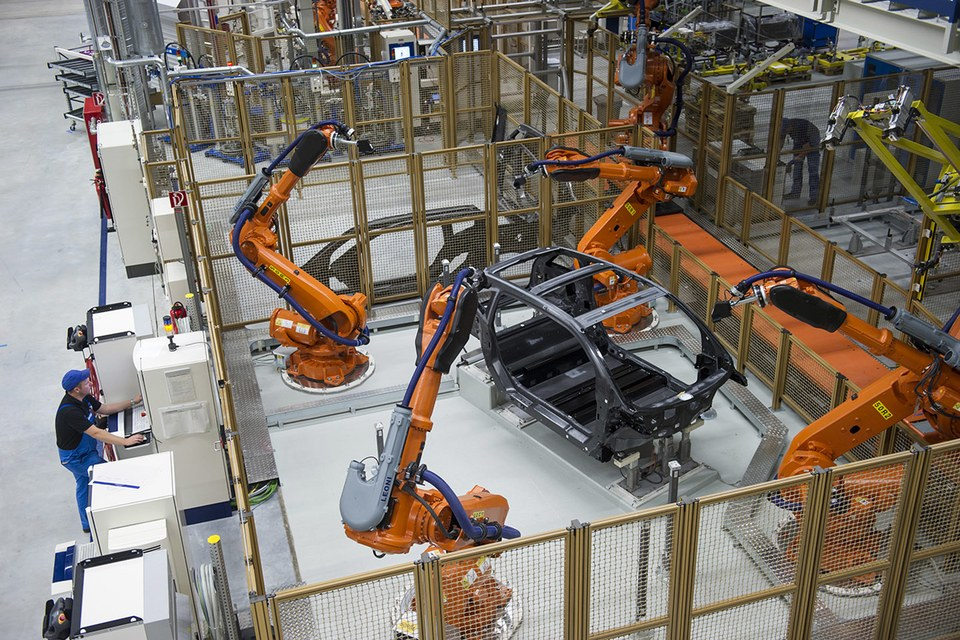
\includegraphics[width = 1.1\linewidth]{tex/figs/robot-factory.jpg}
    \label{fig:mekainside}
    \caption{Fábrica BMW }
\end{figure}
\end{column}
\begin{column}{0.5\textwidth}  %%<--- here
    \begin{itemize}
        \item Repetibilidade
        \item Riscos para o Robô em caso de colisão
        \item Riscos para o Operador
        \item Alto Custo
        \item Rigidez no Sistema
        \item Nenhuma Interação com Pessoas
    \end{itemize}
\end{column}
\end{columns}
\end{frame}

\begin{frame}{Robótica Colaborativa - Sistemas Complacentes}
% Processo de Investigação
\begin{columns}
\begin{column}{0.50\textwidth}
\begin{figure}
    \centering
    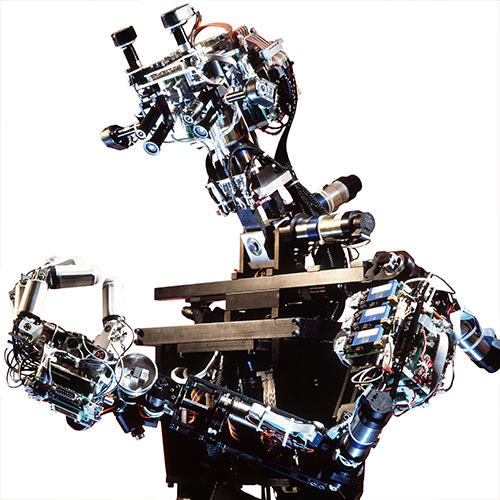
\includegraphics[width = 0.5\linewidth]{tex/figs/cog-mit.jpg}
    \label{fig:mekainside}
    \\{COG (1993)}
\end{figure}

\begin{figure}
    \centering
    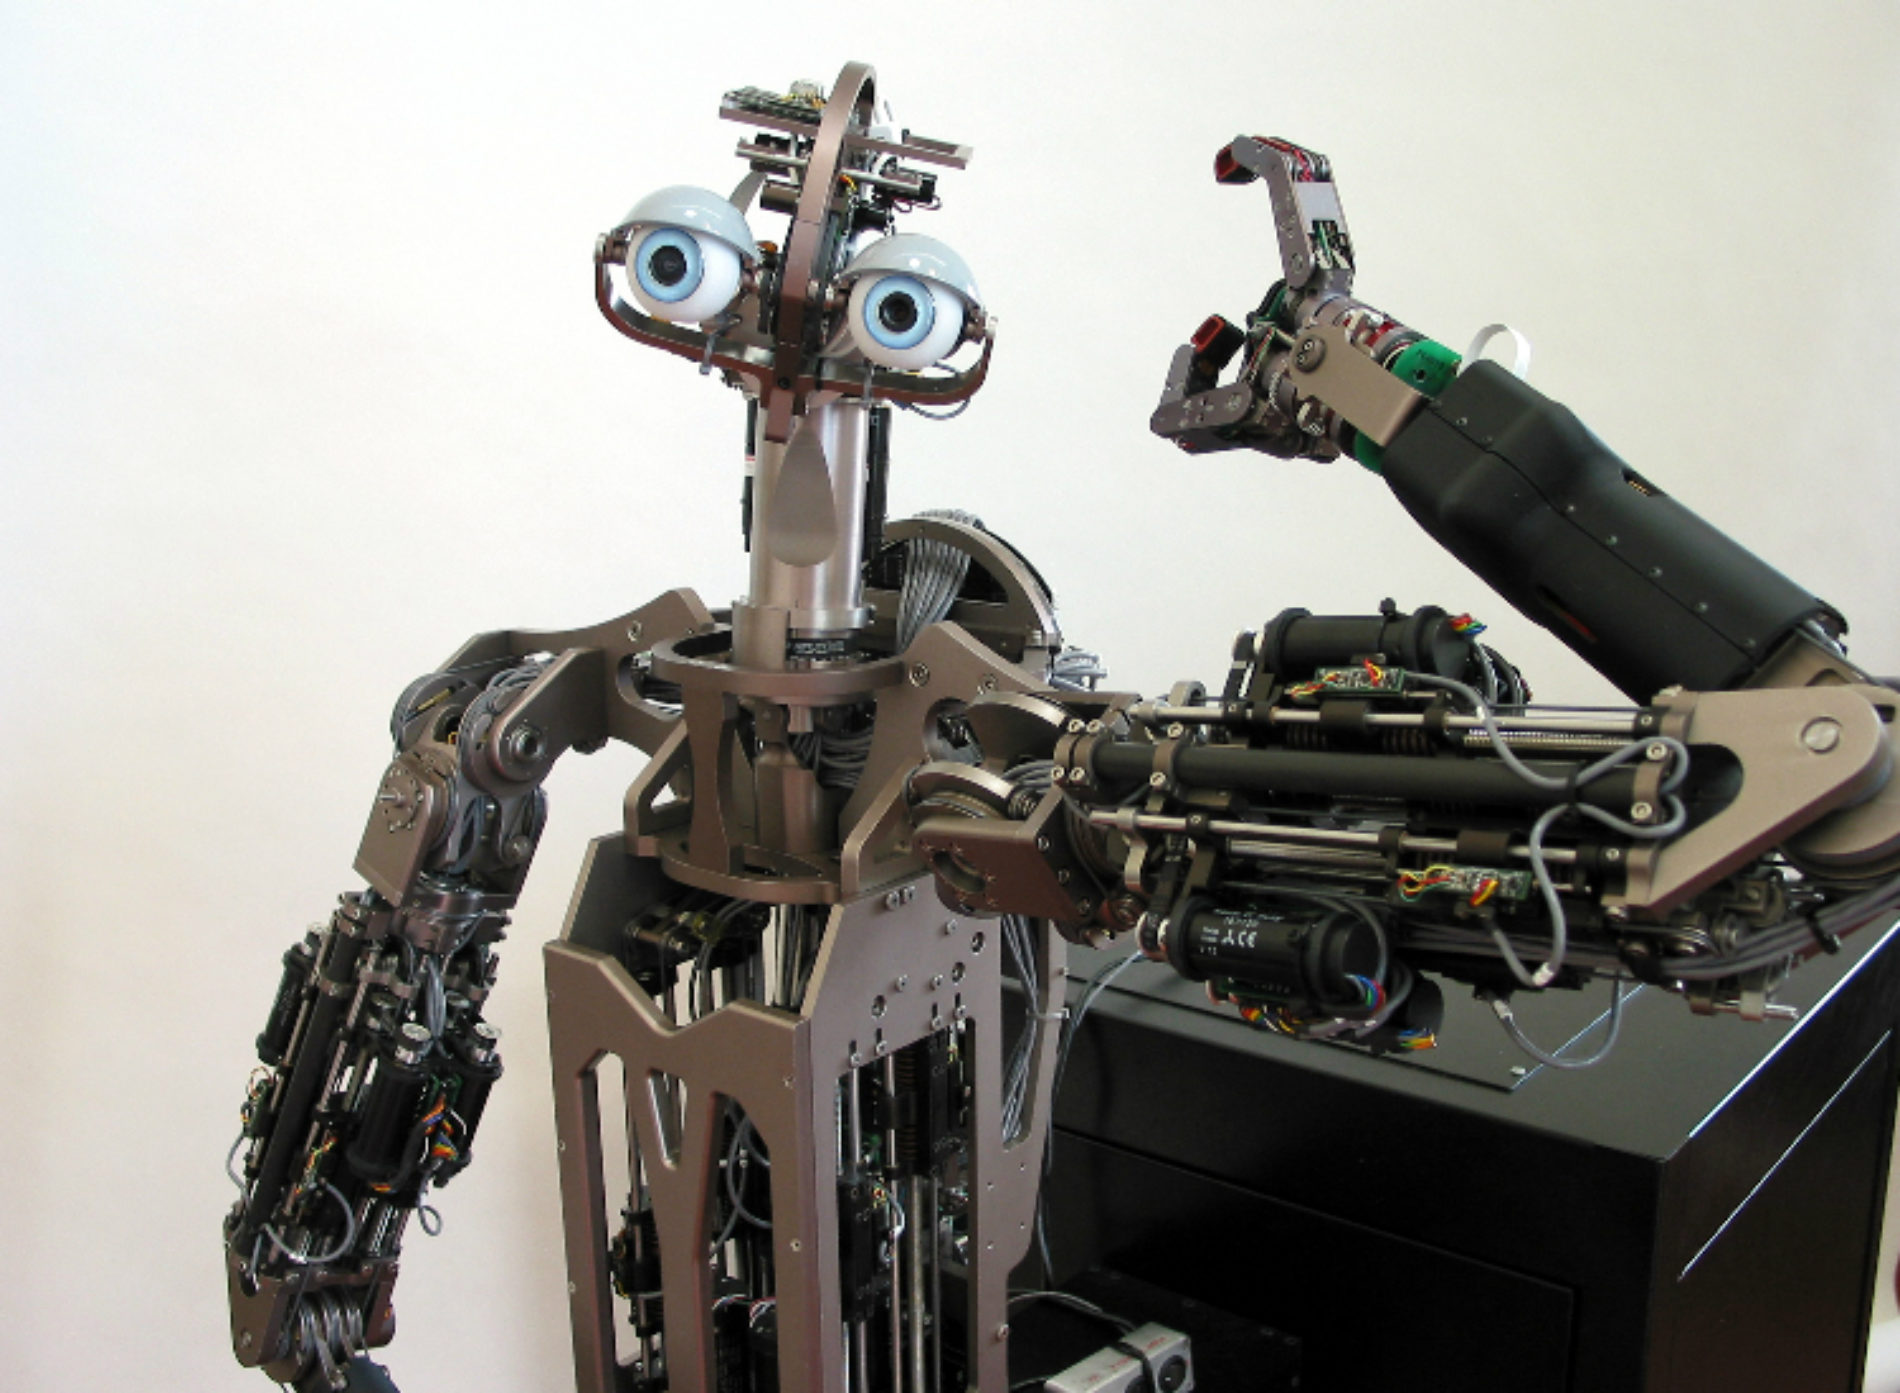
\includegraphics[height = 0.5\linewidth]{tex/figs/domo-foto.jpg}
    \\{DOMO (2003)}
    \label{fig:mekainside}
\end{figure}
\end{column}
\begin{column}{0.5\textwidth}  %%<--- here
\begin{figure}
    \centering
    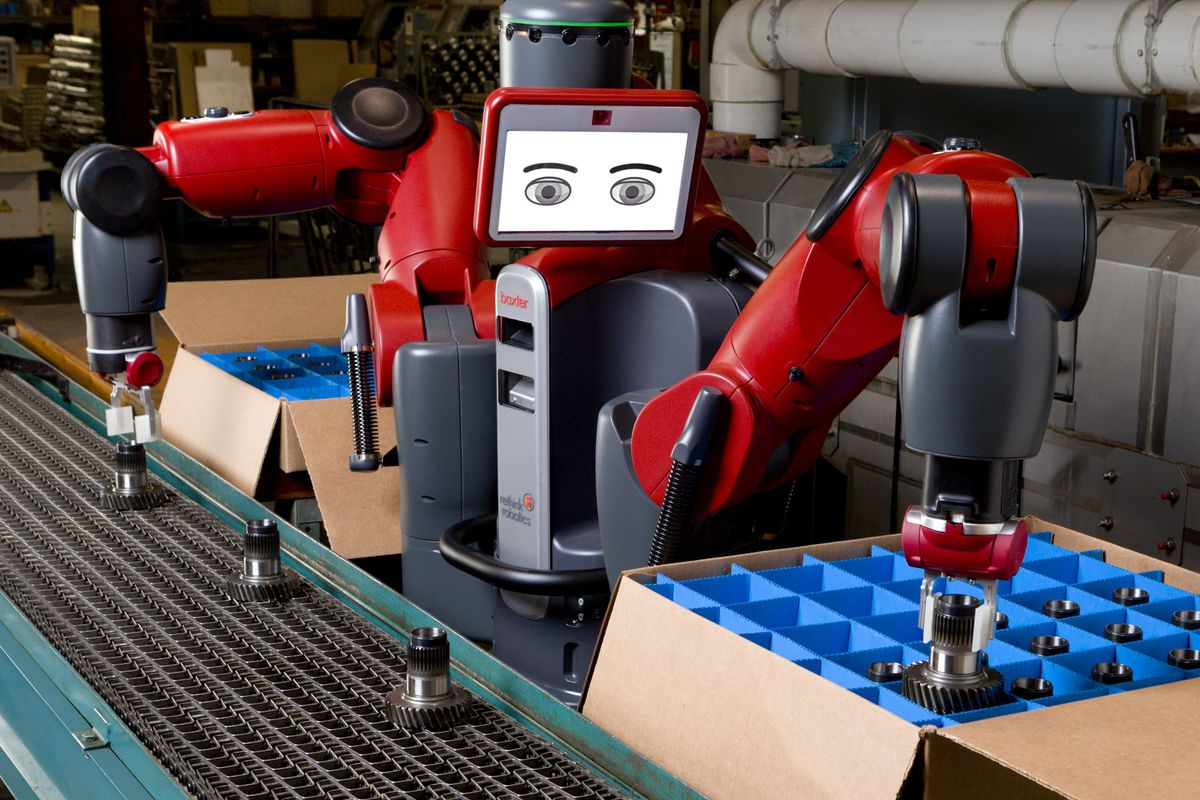
\includegraphics[height = 0.5\linewidth]{tex/figs/baxter_production.jpg}
    \\{Rethink Baxter (2012)}
\end{figure}
\begin{figure}
    \centering
    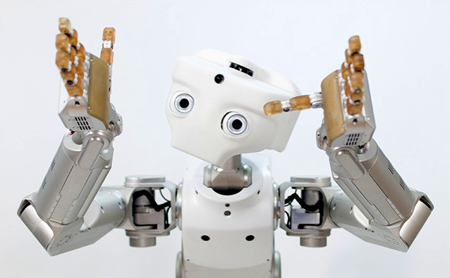
\includegraphics[height = 0.5\linewidth]{tex/figs/meka-robot.png}
    \\{Redwood MEKA A1 (2012)}
\end{figure}
\end{column}
\end{columns}
\end{frame}

%\section{Metodologia}

\begin{frame}{Manipulador Robótico Complacente}
% Processo de Investigação
\begin{figure}
    \centering
    \includegraphics[width = 0.8\linewidth]{tex/figs/meka}
    \caption{Braço Meka A2 do Lara}
    \label{fig:mekainside}
\end{figure}
\end{frame}

\begin{frame}{Problemas}
% Processo de Investigação
\begin{columns}
\begin{column}{0.4\textwidth}  %%<--- here
    \begin{itemize}
        \item Pouca Precisão
        \item Auto Colisão
        \item Pouca Documentação
    \end{itemize}
\end{column}
\begin{column}{0.6\textwidth}
   \begin{figure}
    \centering
    \includegraphics[width = 1.0\linewidth]{tex/figs/meka}
    \label{fig:mekainside}
\end{figure}
\end{column}
\end{columns}
\end{frame}

%\begin{frame}{Processo de Investigação}
% Processo de Investigação
%Processo Heurístico:
%\begin{enumerate}
%    \item Análise e Formulação de Hipóteses
%    \item Formulação de Testes para as Hipóteses
%    \item Avaliação de Hipóteses ( Testes e Estudo teórico )
%\end{enumerate}
%\end{frame}

%\begin{frame}{Processo Científico}
% Processo Cientifico
%\begin{enumerate}
%    \item Perceber Fenômeno
%    \item Descrever através de um sistema lógico
%    \item Reproduzir % Controlar
%\end{enumerate}
%\end{frame}

\section{Conceitos Teóricos}
\subsection{Controle de Manipuladores Robóticos}

\begin{frame}{Modelagem}

\begin{columns}
\begin{column}{0.4\textwidth}  %%<--- here
Modelo Braço Robótico:
\begin{itemize}
    \item Ação conjunta de vários atuadores
    \item Cinemática Direta
    \item Cinemática Inversa
\end{itemize}
\end{column}
\begin{column}{0.6\textwidth}
\begin{figure}
    \centering
    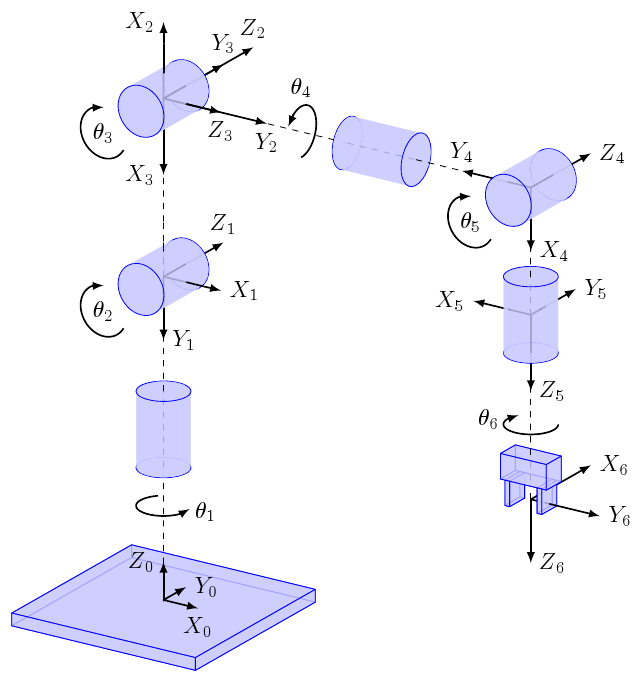
\includegraphics[width = 0.8\linewidth]{tex/figs/robotkine.png}
    \caption{Representação Cinemática}
    \label{fig:mekainside}
\end{figure}
\end{column}
\end{columns}
\end{frame}

%\begin{frame}{Controle Manipuladores}
% Processo Cientifico
% https://i.stack.imgur.com/nwvIN.png
%\begin{figure}
%    \centering
%    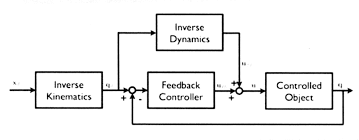
\includegraphics[width = 0.9\linewidth]{tex/figs/controlkine.png}
%    \caption{Controle Cinemático}
%    \label{fig:mekainside}
%\end{figure}
%\end{frame}

\begin{frame}{Meka A2 Arm}
% Processo Cientifico
Componentes: sistemas mecânicos, eletrônicos, computacionais
\begin{figure}
    \centering
    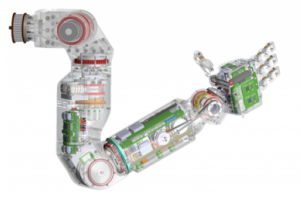
\includegraphics[width = 0.8\linewidth]{tex/figs/meka-arm-inside}
    \caption{Representação dos Componentes Internos do Meka}
    \label{fig:mekainside}
\end{figure}
\end{frame}

\subsection{Arquitetura do Sistema do Meka}

\begin{frame}{Atuadores Série Elásticos}
% Processo Cientifico
Complacência em cada Junta:
\begin{figure}
    \centering
    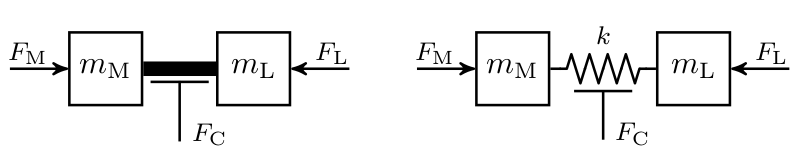
\includegraphics[width = 0.8\linewidth]{tex/figs/sea_ulrich.png}
    \caption{Atuador Rígido (Esquerda) e Atuador Série Elástico}
    \label{fig:mekainside}
\end{figure}
A diferença de força entre a carga e o motor pode ser expresso pela Lei de Hooke:
\begin{equation}
    F = -K\Delta X
\end{equation}
\end{frame}

\begin{frame}{Mecânica: Atuadores Série Elásticos}
% Processo Cientifico
\begin{itemize}
    \item Uso de Sensores de Posição para medir o torque
    \item Controle de Torque com Precisão
    \item Controle de Complacência
\end{itemize}
\begin{figure}
    \centering
    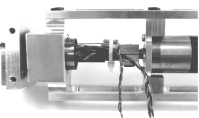
\includegraphics[width = 0.6\linewidth]{tex/figs/sea_pratt.png}
    \caption{Atuador Série Elástico feito por Pratt}
    \label{fig:mekainside}
\end{figure}
\end{frame}

\begin{frame}{Mecânica: Pulso Diferencial}
\begin{columns}
\begin{column}{0.6\textwidth}
\begin{figure}
    \centering
    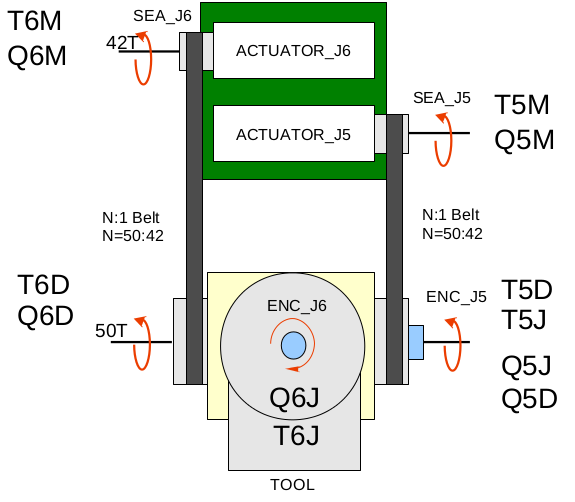
\includegraphics[width = 0.6\linewidth]{tex/figs/meka_wrist.png}
    \caption{Pulso Diferencial}
    \label{fig:m3arch}
\end{figure}
\end{column}
\begin{column}{0.4\textwidth}  %%<--- here
\begin{itemize}
    \item Uso de dois motores para movimentação do pulso
\end{itemize}
\end{column}
\end{columns}
\end{frame}

\begin{frame}{Arquitetura Meka}
\begin{figure}
    \centering
    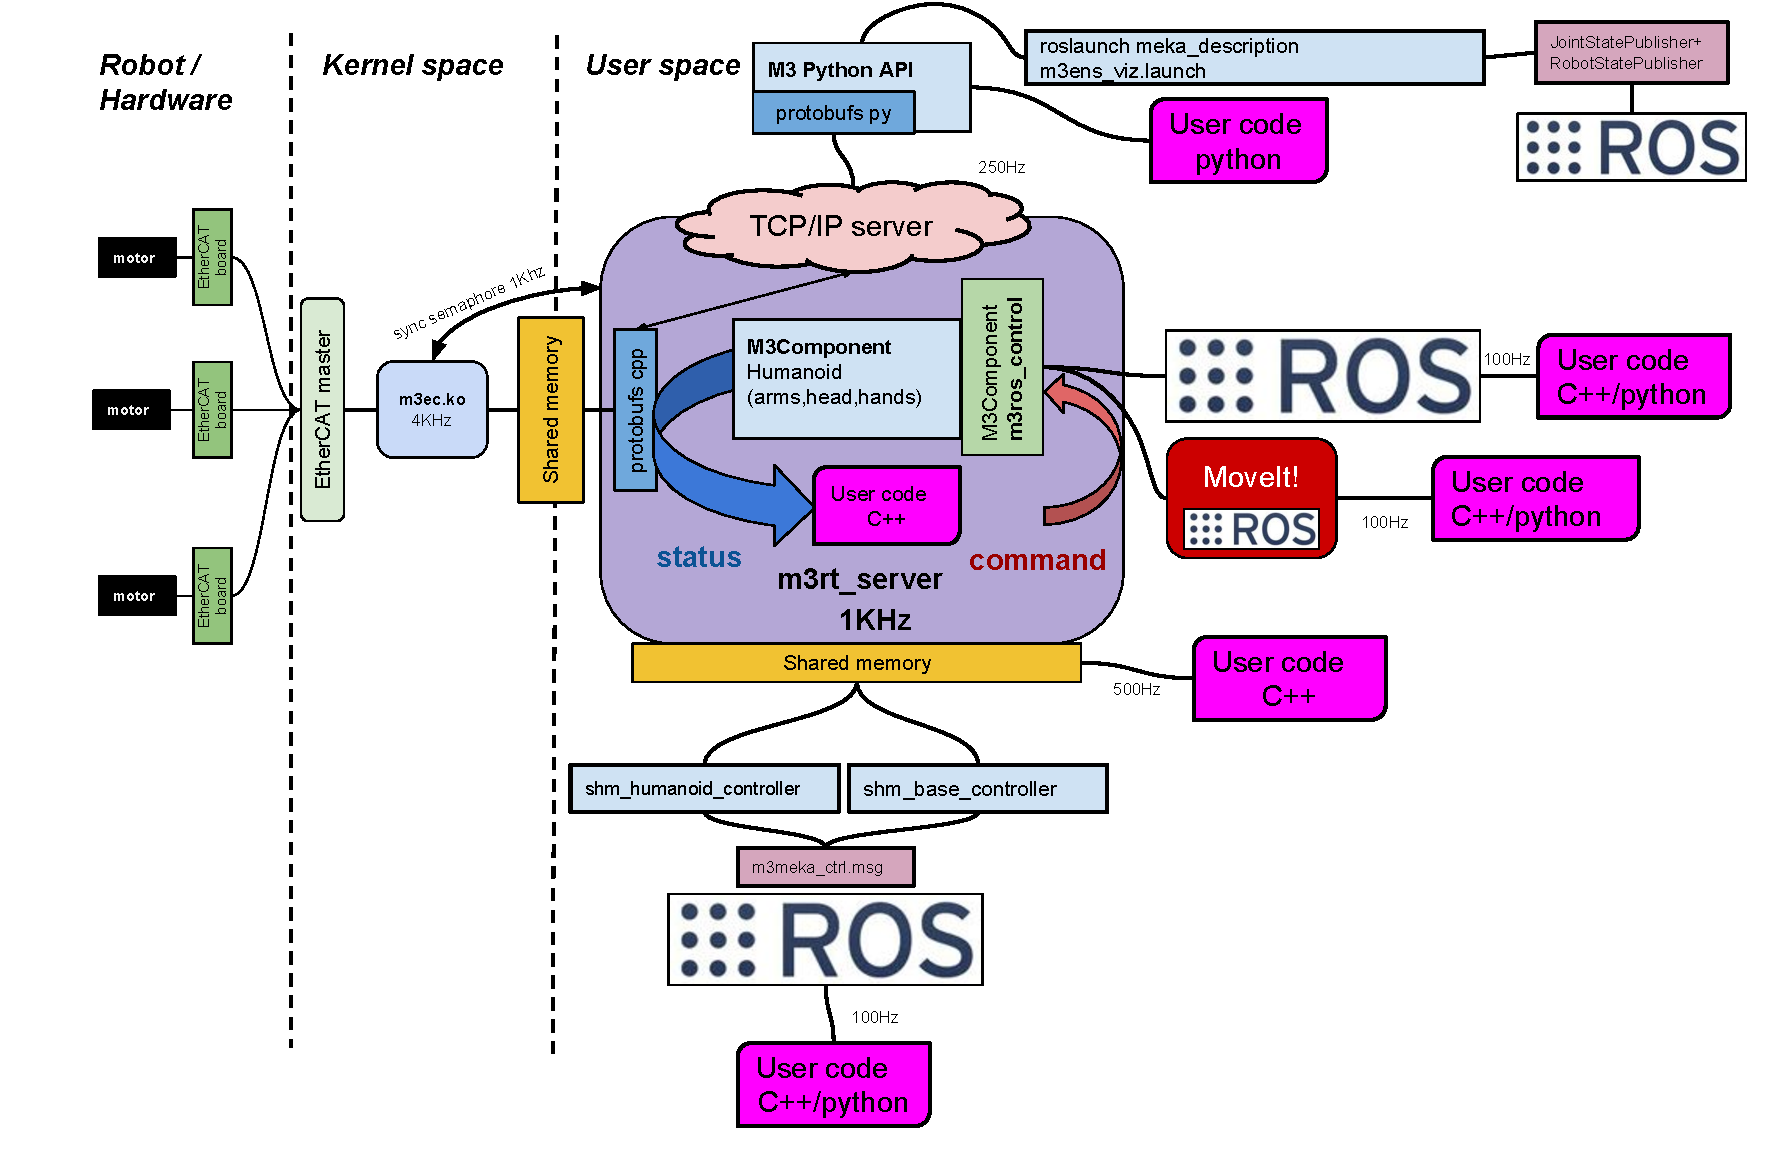
\includegraphics[width = \linewidth]{tex/figs/m3_arch}
    \caption{Diagrama da Arquitetura do Robô}
    \label{fig:m3_arch}
\end{figure}
\end{frame}

\begin{frame}{Arquitetura M3}
\begin{columns}
\begin{column}{0.6\textwidth}
\begin{figure}
    \centering
    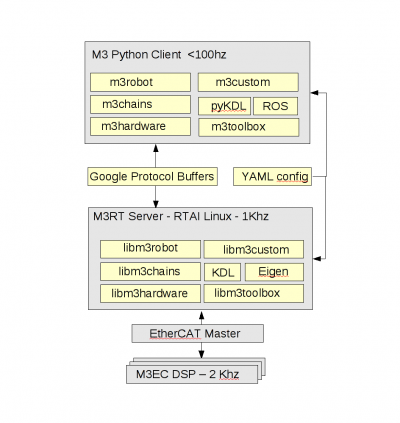
\includegraphics[width = \linewidth]{tex/figs/m3arch}
    \caption{Sistema do Controle M3}
    \label{fig:m3arch}
\end{figure}
\end{column}
\begin{column}{0.4\textwidth}  %%<--- here
Desafios:
\begin{itemize}
    \item Pouca Documentação
    \item Estrutura Complexa
\end{itemize}
\end{column}
\end{columns}
\end{frame}

\begin{frame}{Arquitetura Controladores}
\begin{figure}
    \centering
    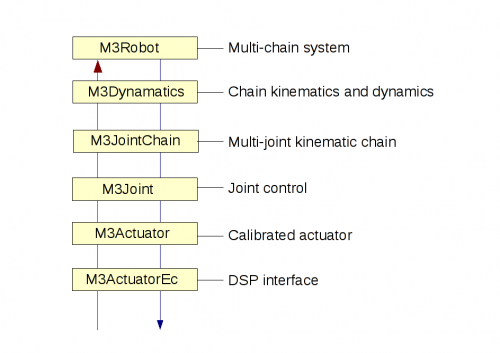
\includegraphics[width = 0.8\linewidth]{tex/figs/controlarch.png}
    \caption{Arquitetura Controladores}
    \label{fig:m3arch}
\end{figure}
\end{frame}

\subsection{Critério de Desempenho}

\begin{frame}{Desempenho de Sistema de Controle}
\begin{figure}
    \centering
    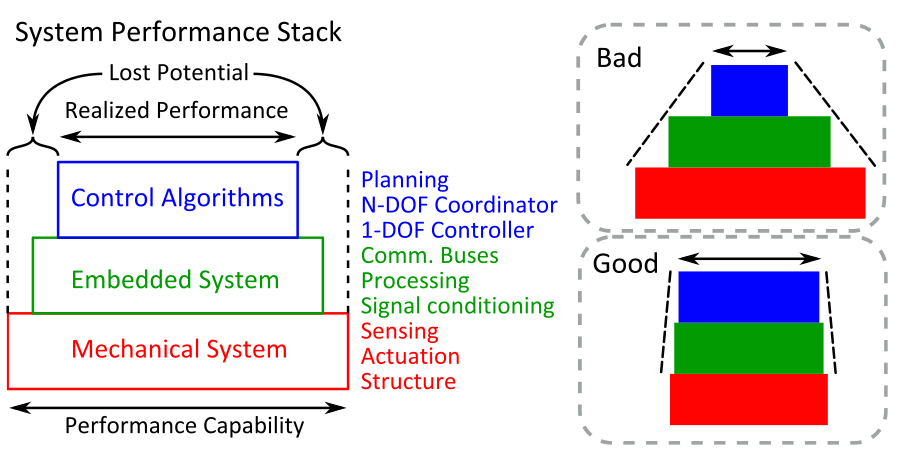
\includegraphics[width = 0.9\linewidth]{tex/figs/system_perfomance.png}
    \caption{Representação da Capacidade de Desempenho}
    \label{fig:system_perfomance}
\end{figure}
\end{frame}

\section{Resultados}
\subsection{Avaliação Preliminar}
\begin{frame}{Atuadores e Sensores}
\begin{block}{Atuadores}
    \begin{table}[H]
    \centering
    \tiny
    \caption{Especificação Preliminar dos Atuadores, adaptado de \cite{mekaguide}}
    \begin{tabular}{c|ccccccc}
         \hline
         A2.R4 Spec & $\theta_0$ & $\theta_1$ & $\theta_2$ & $\theta_3$ & $\theta_4$ & $\theta_5$ & $\theta_6$\\
         \hline
         Torque Cont  (nM)     & 14.6   & 16.7   & 9.6    & 9.6    & 1.9    & 2.3   & 2.3 \\
         Torque Mom (nM)      & 40.0   & 40.0   & 20.0   & 20.0   & 4.0    & 8.0   & 8.0 \\
         Rigidez (Nm/rad)     & 417.0  & 417.0  & 190.0  & 190.0  & 23.0   & 46.0  & 46.0 \\
         Max Vel (Rad/s)      & 4.6    & 4.6    & 4.5    & 4.5    & \textbf{\color{blue}2.0}   & 3.4   & 3.4 \\
         \hline
    \end{tabular}
    \label{tab:a2armActuationDoc}
\end{table}
\end{block}
\begin{block}{Sensores}
\begin{itemize}
    \item Torque e Posição: ContLec Vert-X13 Encoder Absoluto; 14 bits (0.02 graus de precisão)
    \item Percepção diferente de torque por junta ($\tau = -K\Delta x $)
\end{itemize}
\end{block}
\end{frame}

\begin{frame}{Sistema Embarcado}
\begin{columns}
\begin{column}{0.5\textwidth}  %%<--- here
\begin{figure}
    \centering
    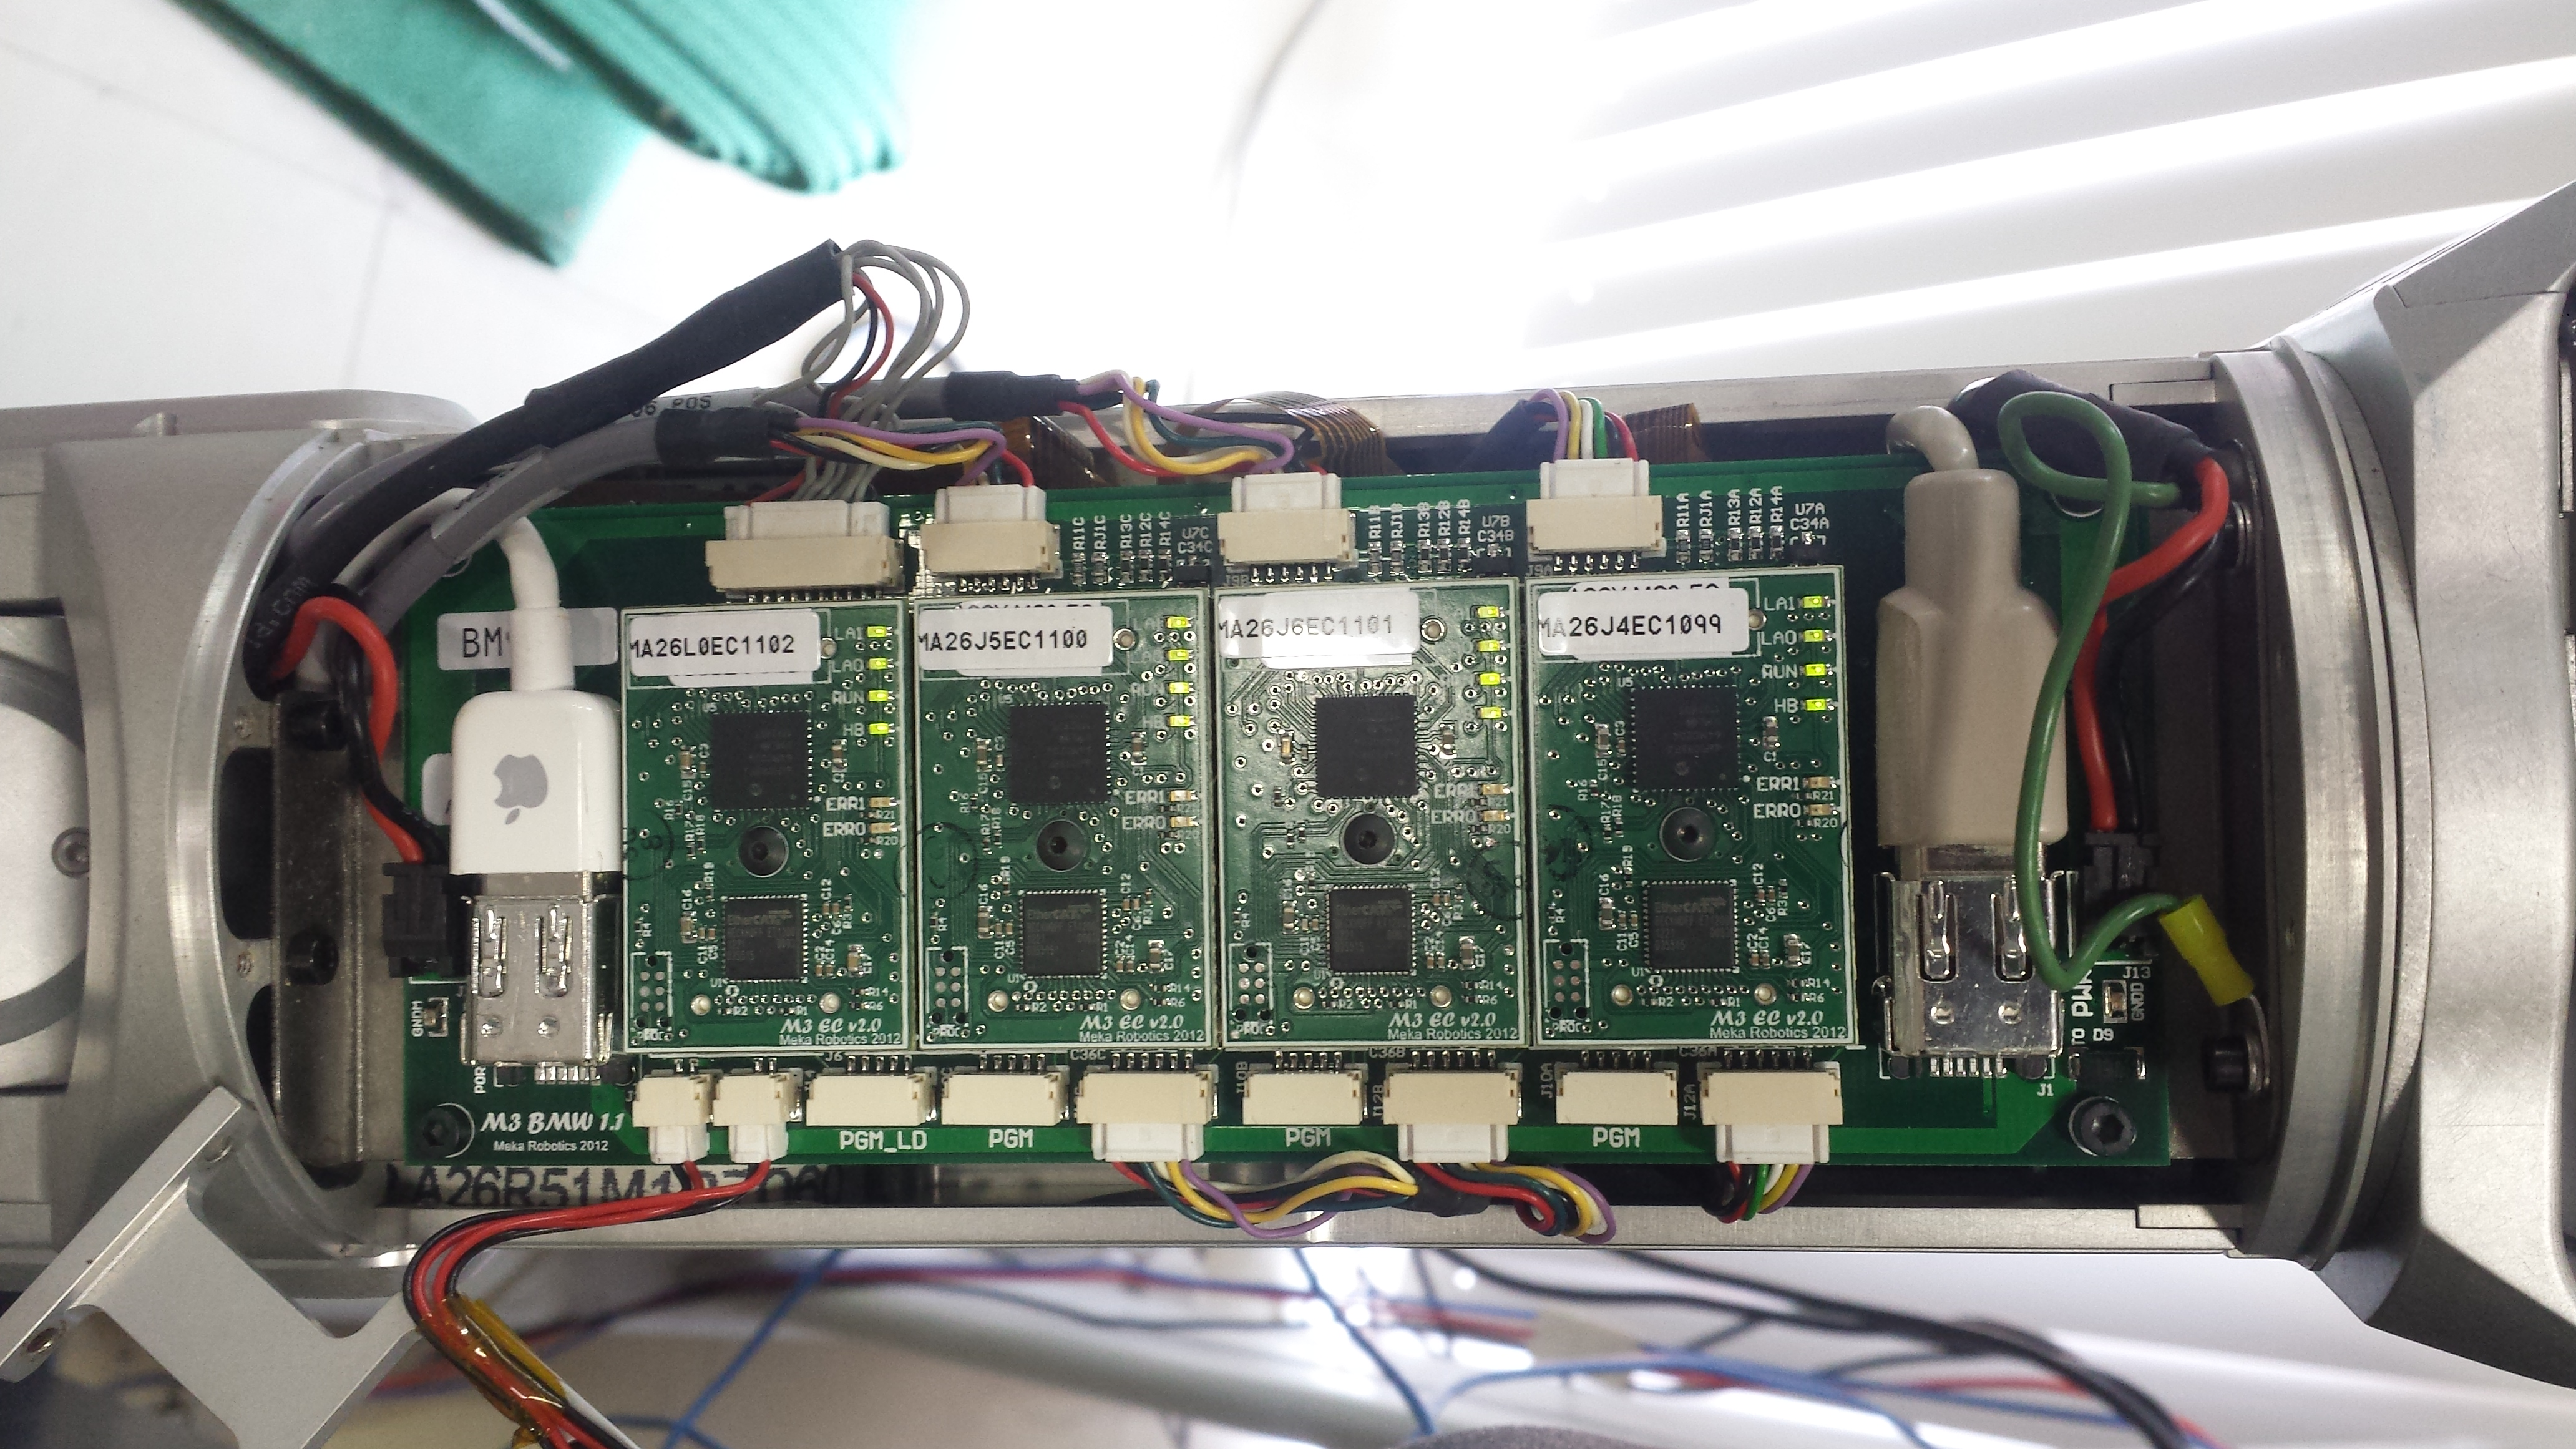
\includegraphics[height = 0.7\linewidth, angle=270]{tex/figs/dsp-control-wrist.jpg}
    \label{fig:mekawristinside}
\end{figure}
\end{column}
\begin{column}{0.5\textwidth}
\begin{itemize}
    \item DSP: Interface Atuadores e Sensores
    \item EtherCAT ( Protocolo de Comunicação Rápida )
    \item PC: intel i7, 8GB Linux com Kernel RTOS
\end{itemize}
\end{column}
\end{columns}
\end{frame}

\subsection{Controladores de Juntas}

\begin{frame}{Controle de Rigidez das Juntas}
Experimento de Resposta com um valor fixo de referência:
\begin{columns}
\begin{column}{0.5\textwidth}
   \begin{figure}
    \centering
    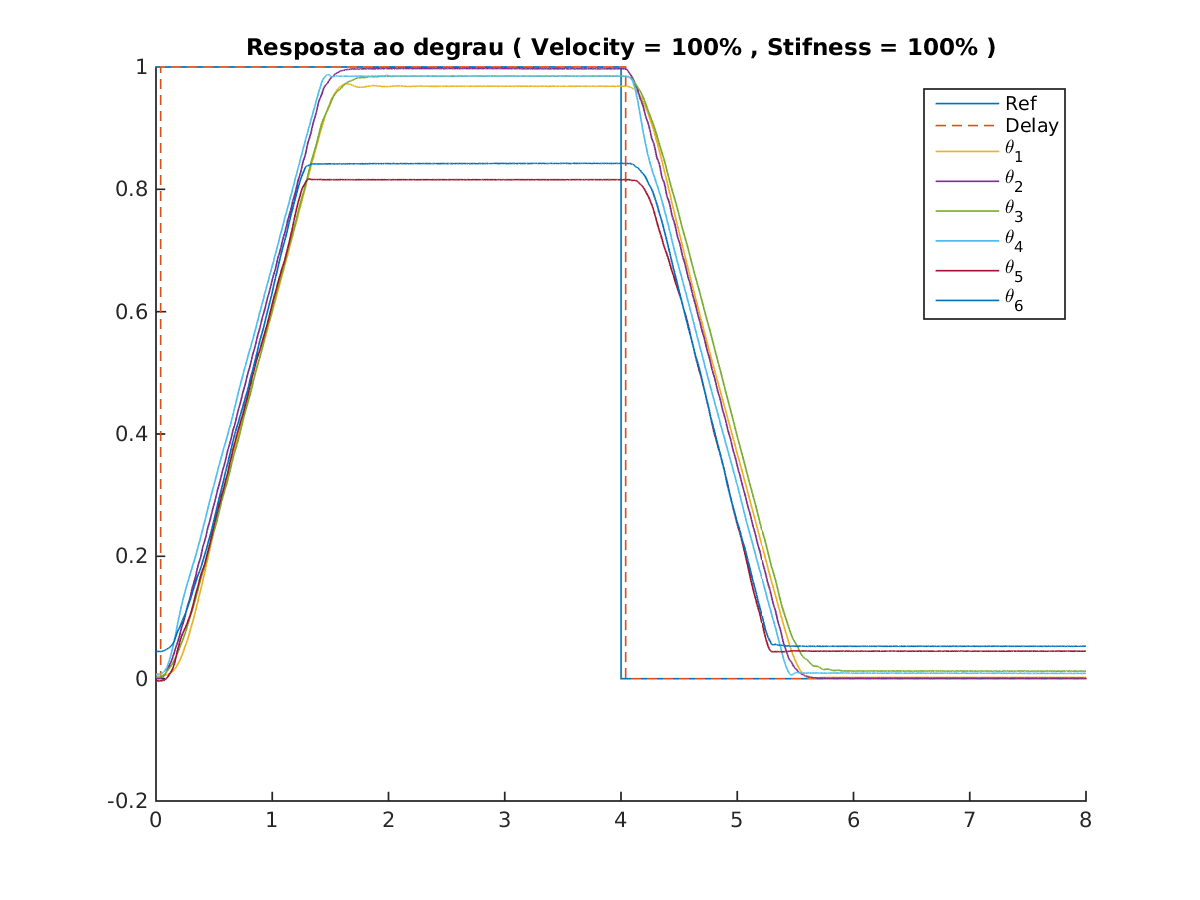
\includegraphics[width = \linewidth]{tex/figs/jointIdentification_exp1v100v100.png}
    \caption{Rigidez 100\%}
    \label{fig:mekademo}
\end{figure}
\end{column}
\begin{column}{0.5\textwidth}  %%<--- here
    \begin{figure}
    \centering
    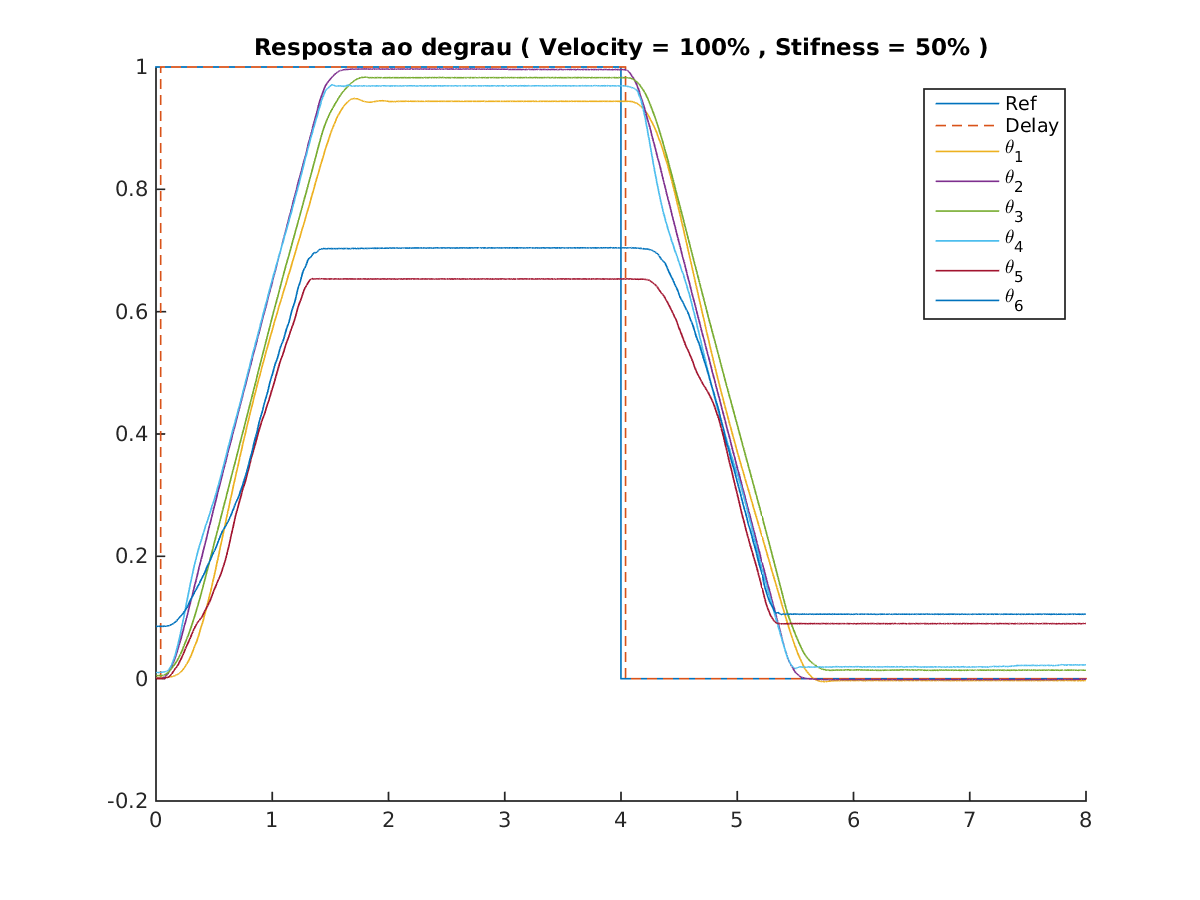
\includegraphics[width = \linewidth]{tex/figs/jointIdentification_exp2v100v50.png}
    \caption{Rigidez 50\%}
    \label{fig:mekademo}
\end{figure}
\end{column}
\end{columns}
\end{frame}

\begin{frame}{Controle de Rigidez das Juntas}
Experimento de Resposta com um valor fixo de referência:
\begin{columns}
\begin{column}{0.5\textwidth}
   \begin{figure}
    \centering
    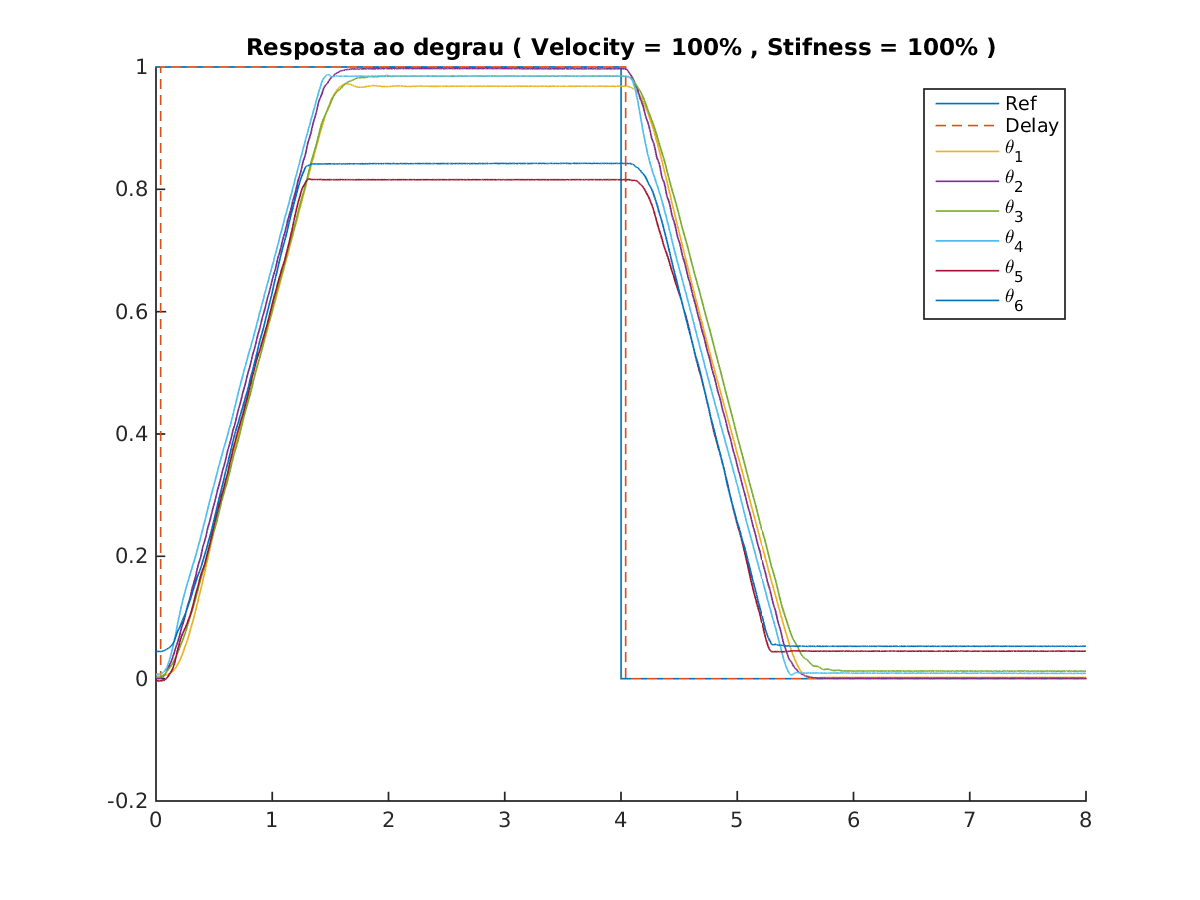
\includegraphics[width = \linewidth]{tex/figs/jointIdentification_exp1v100v100.png}
    \caption{Velocidade 100\%}
    \label{fig:mekademo}
\end{figure}
\end{column}
\begin{column}{0.5\textwidth}  %%<--- here
    \begin{figure}
    \centering
    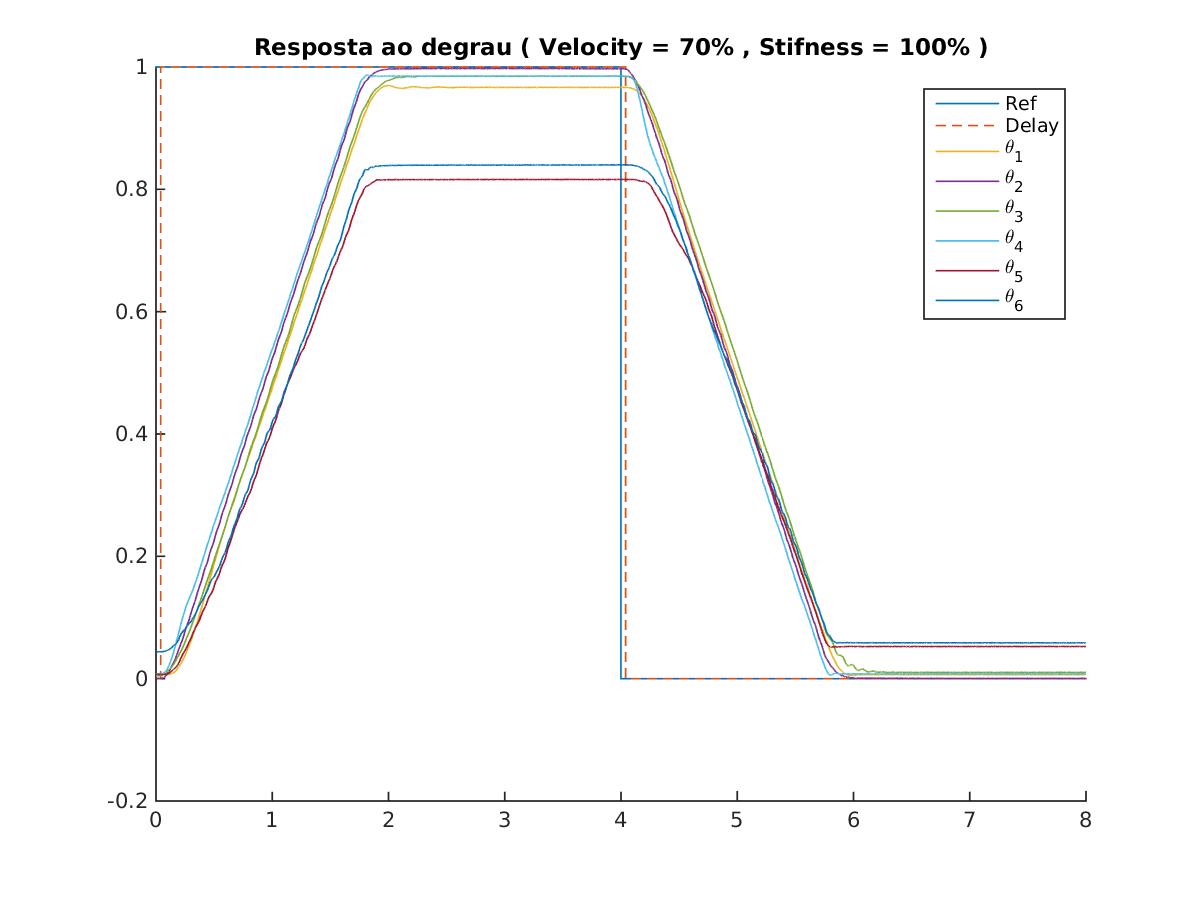
\includegraphics[width = \linewidth]{tex/figs/jointIdentification_exp3v70v100.png}
    \caption{Velocidade 70\%}
    \label{fig:mekademo}
\end{figure}
\end{column}
\end{columns}
\end{frame}

\subsection{Controladores Cinemáticos}

\begin{frame}{Trajetória em Linha Reta - dt = 10ms}
   \begin{figure}
    \centering
    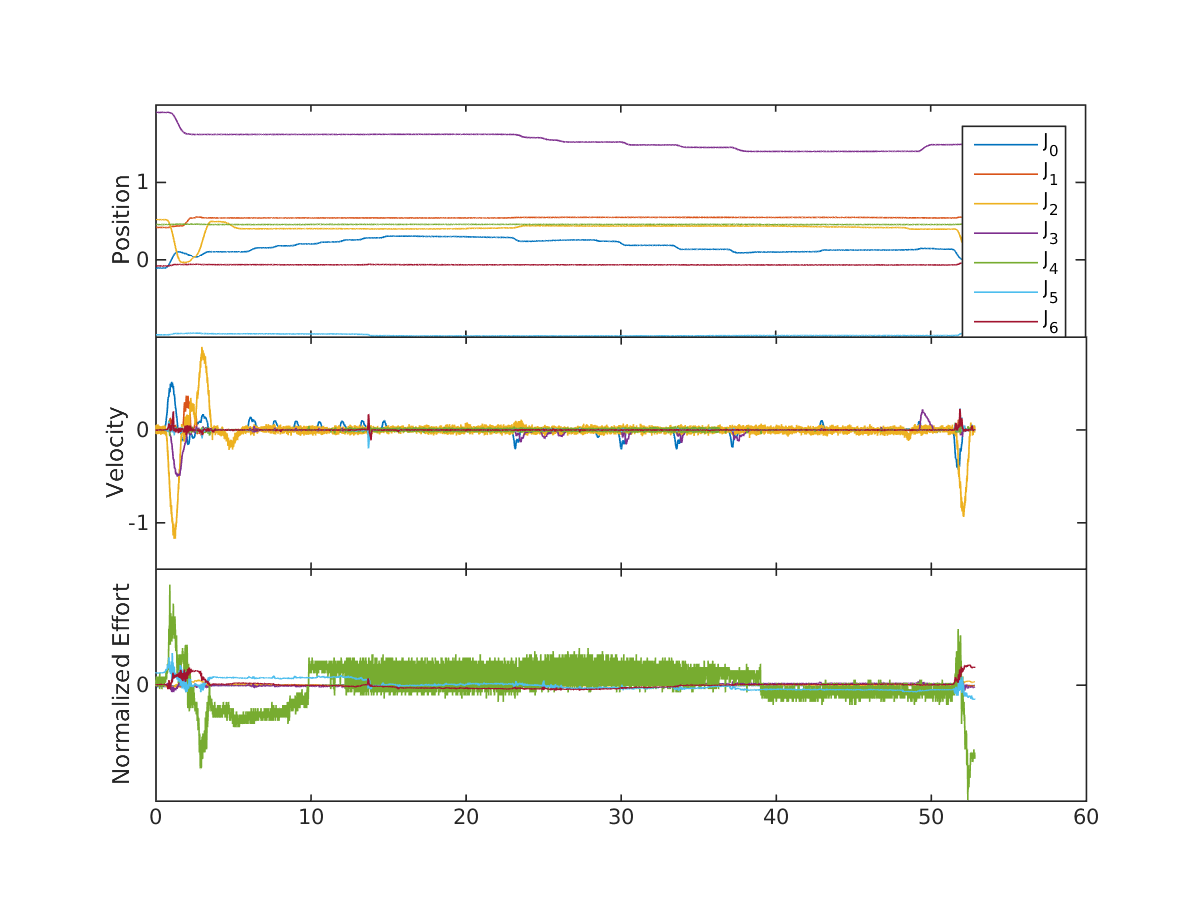
\includegraphics[width = 0.9\linewidth]{tex/figs/moveUp1stateEvalv70s10.png}
    \label{fig:mekademo}
\end{figure}
\end{frame}

\begin{frame}{Trajetória em Linha Reta - dt = 2ms}
   \begin{figure}
    \centering
    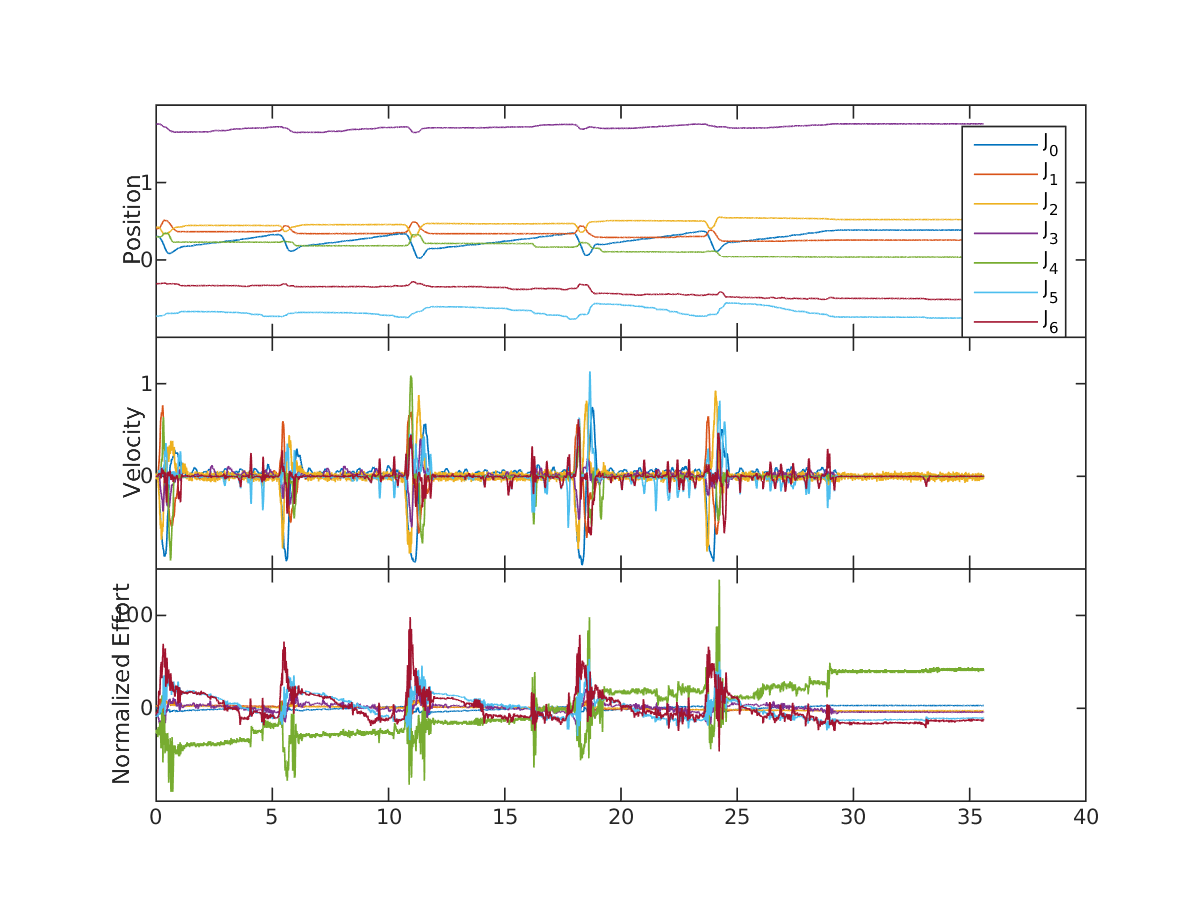
\includegraphics[width = 0.9\linewidth]{tex/figs/moveUp3stateEvalv70s50.png}
    \label{fig:mekademo}
\end{figure}
\end{frame}

\begin{frame}{Estudo Velocidade e Torque - V = 100\%}
   \begin{figure}
    \centering
    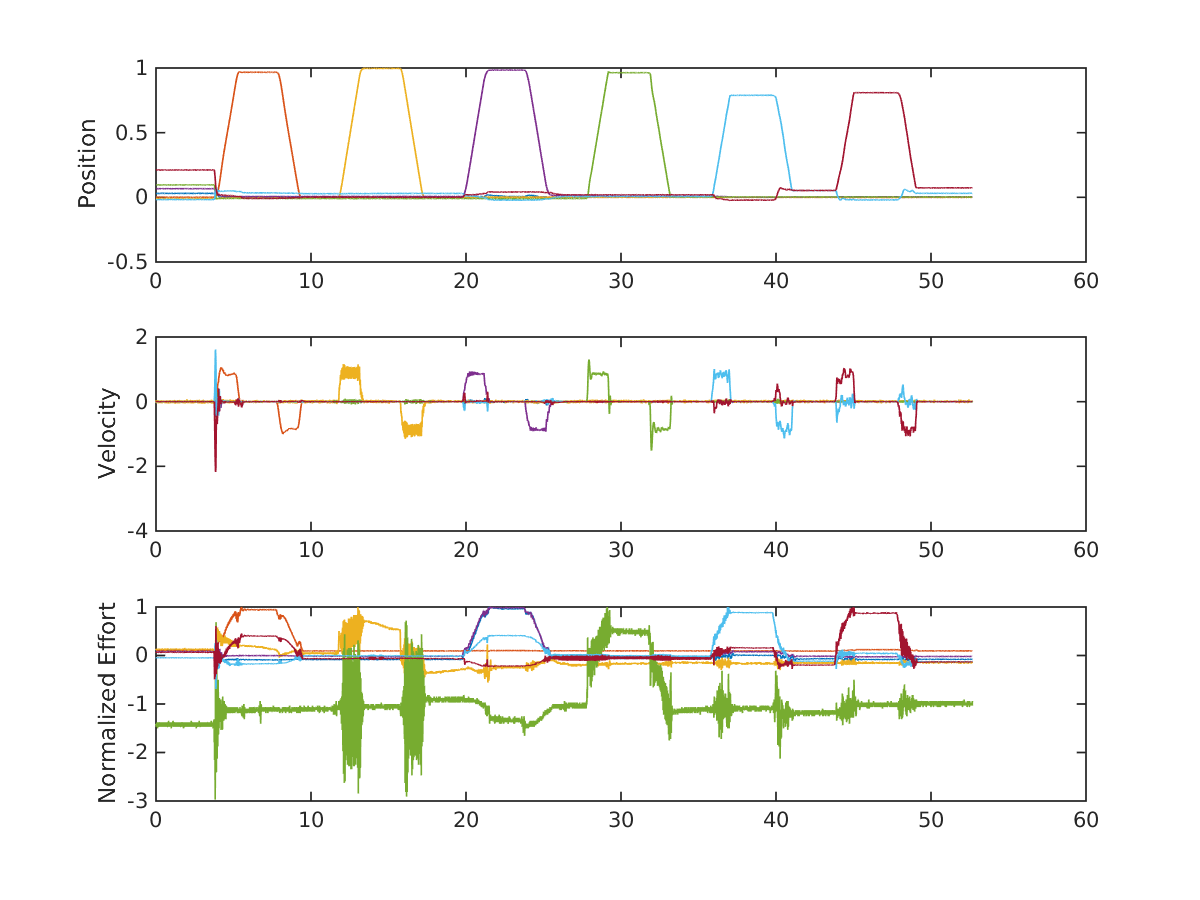
\includegraphics[width = 0.9\linewidth]{tex/figs/jointIdentificationFullSpeed_stiff90p.png}
    \label{fig:mekademo}
\end{figure}
\end{frame}

\begin{frame}{Estudo Velocidade e Torque - V = 10\%}
   \begin{figure}
    \centering
    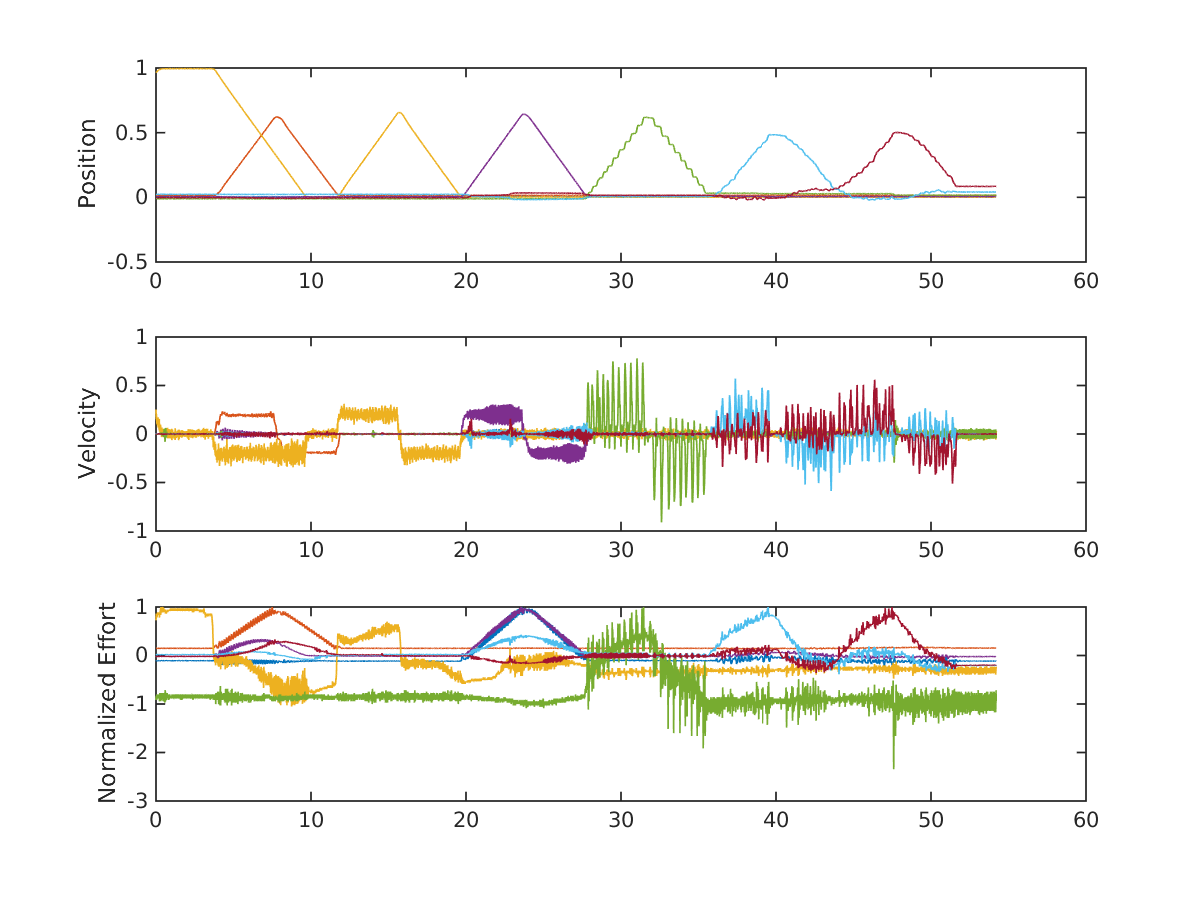
\includegraphics[width = 0.9\linewidth]{tex/figs/jointIdentificationSpeed10p_stiff90p2.png}
    \label{fig:mekademo}
\end{figure}
\end{frame}

\begin{frame}{Controle de Rigidez das Juntas}
Experimento de Resposta com um valor fixo de referência:
\begin{columns}
\begin{column}{0.5\textwidth}
   \begin{figure}
    \centering
    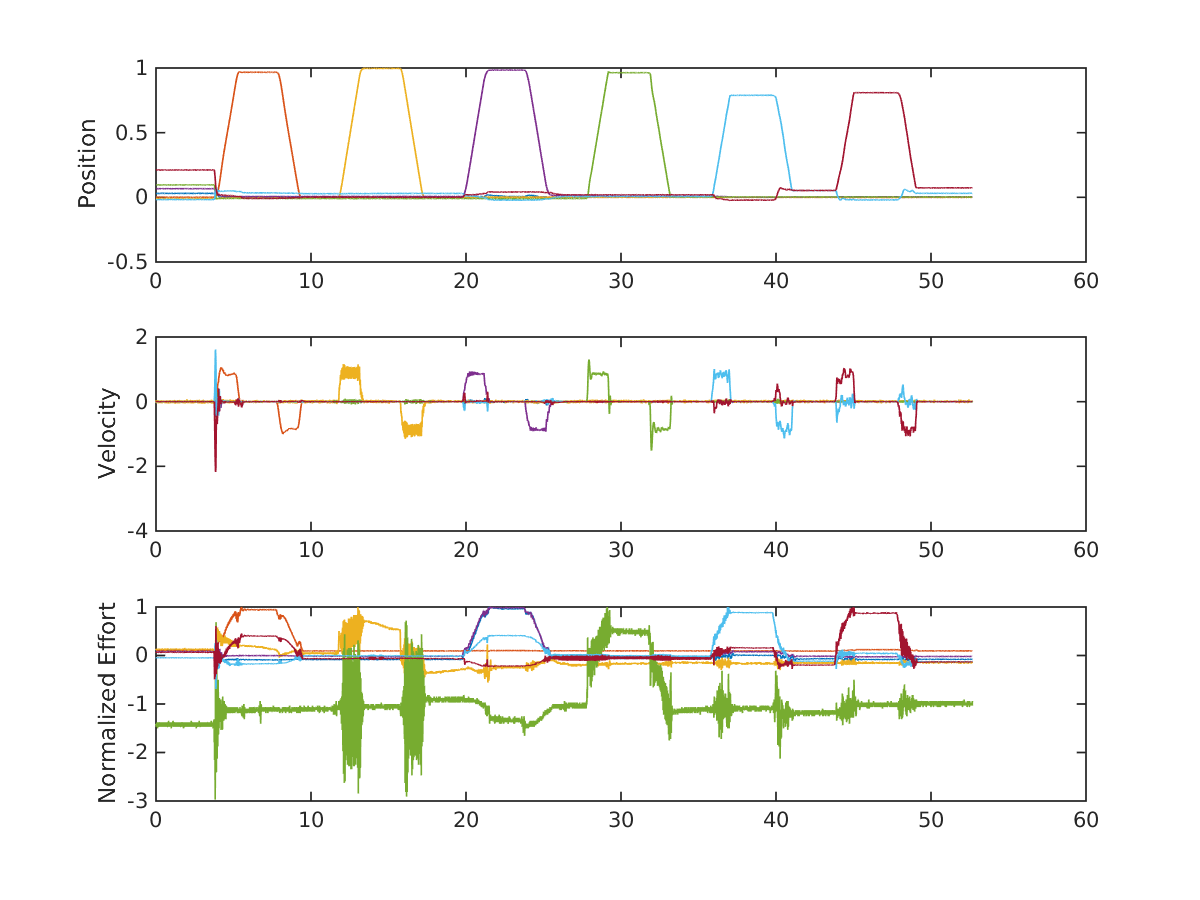
\includegraphics[width = \linewidth]{tex/figs/jointIdentificationFullSpeed_stiff90p.png}
    \caption{Velocidade 100\%}
    \label{fig:mekademo}
\end{figure}
\end{column}
\begin{column}{0.5\textwidth}  %%<--- here
    \begin{figure}
    \centering
    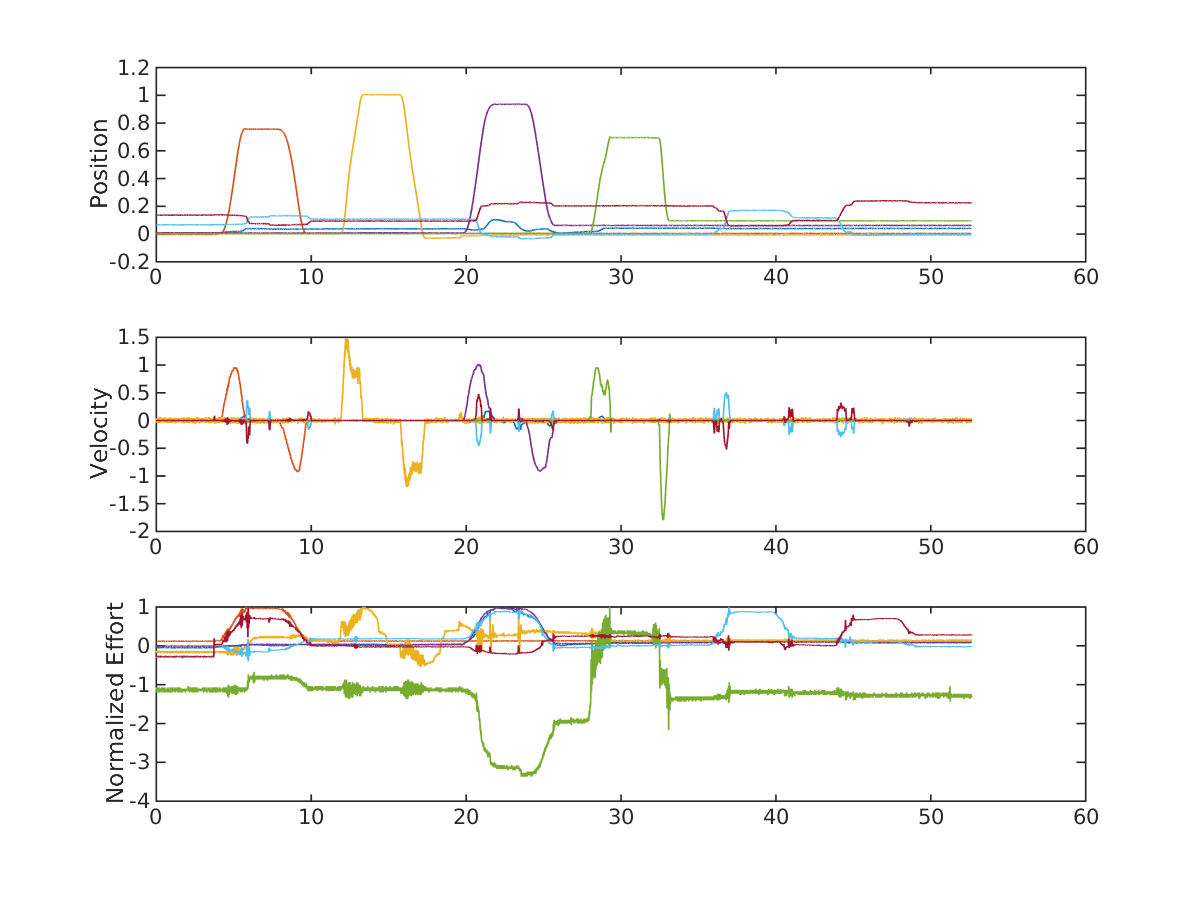
\includegraphics[width = \linewidth]{tex/figs/jointIdentificationFullSpeed_stiff10p.png}
    \caption{Velocidade 70\%}
    \label{fig:mekademo}
\end{figure}
\end{column}
\end{columns}
\end{frame}

\begin{frame}{Trajetória Quadrado - Resposta Controladores de Junta}
   \begin{figure}
    \centering
    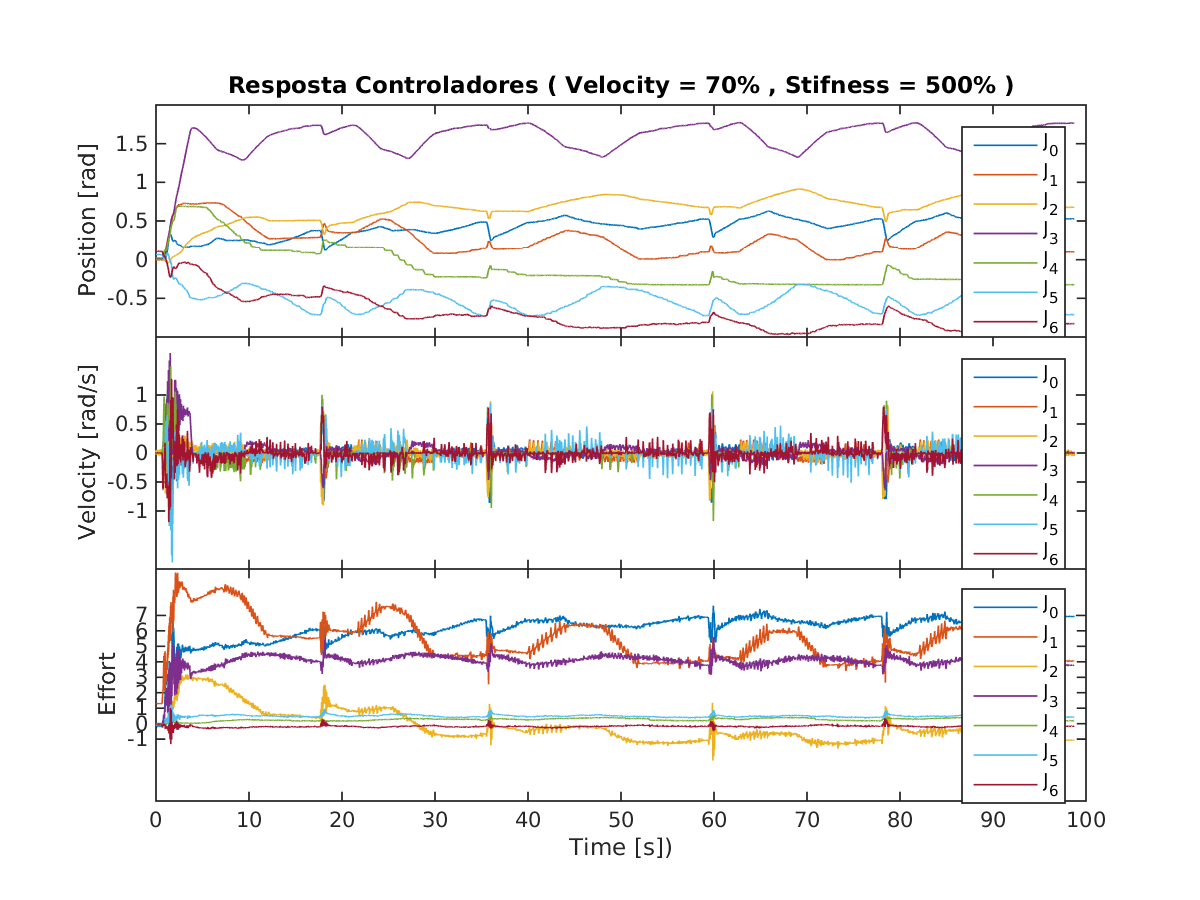
\includegraphics[width = 0.9\linewidth]{tex/figs/squareStifff3stateEvalv70s500.png}
    \label{fig:mekademo}
\end{figure}
\end{frame}

\begin{frame}{Estudo Trajetória Quadrado}
Resposta Juntas do Ombro
\begin{columns}
\begin{column}{0.5\textwidth}
   \begin{figure}
    \centering
    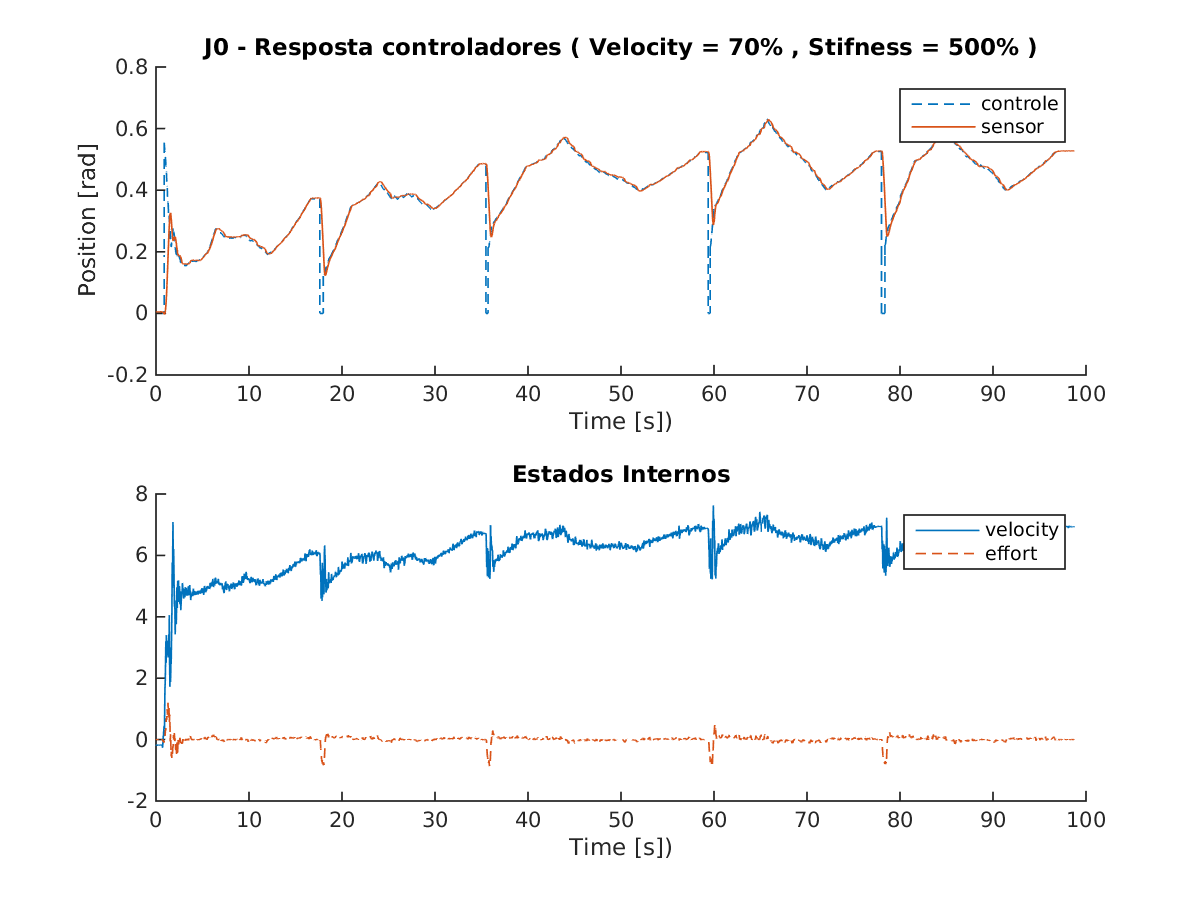
\includegraphics[width = \linewidth]{tex/figs/squareStiffJ3stateEval_J0v70s500.png}
    \label{fig:mekademo}
\end{figure}
\end{column}
\begin{column}{0.5\textwidth}  %%<--- here
    \begin{figure}
    \centering
    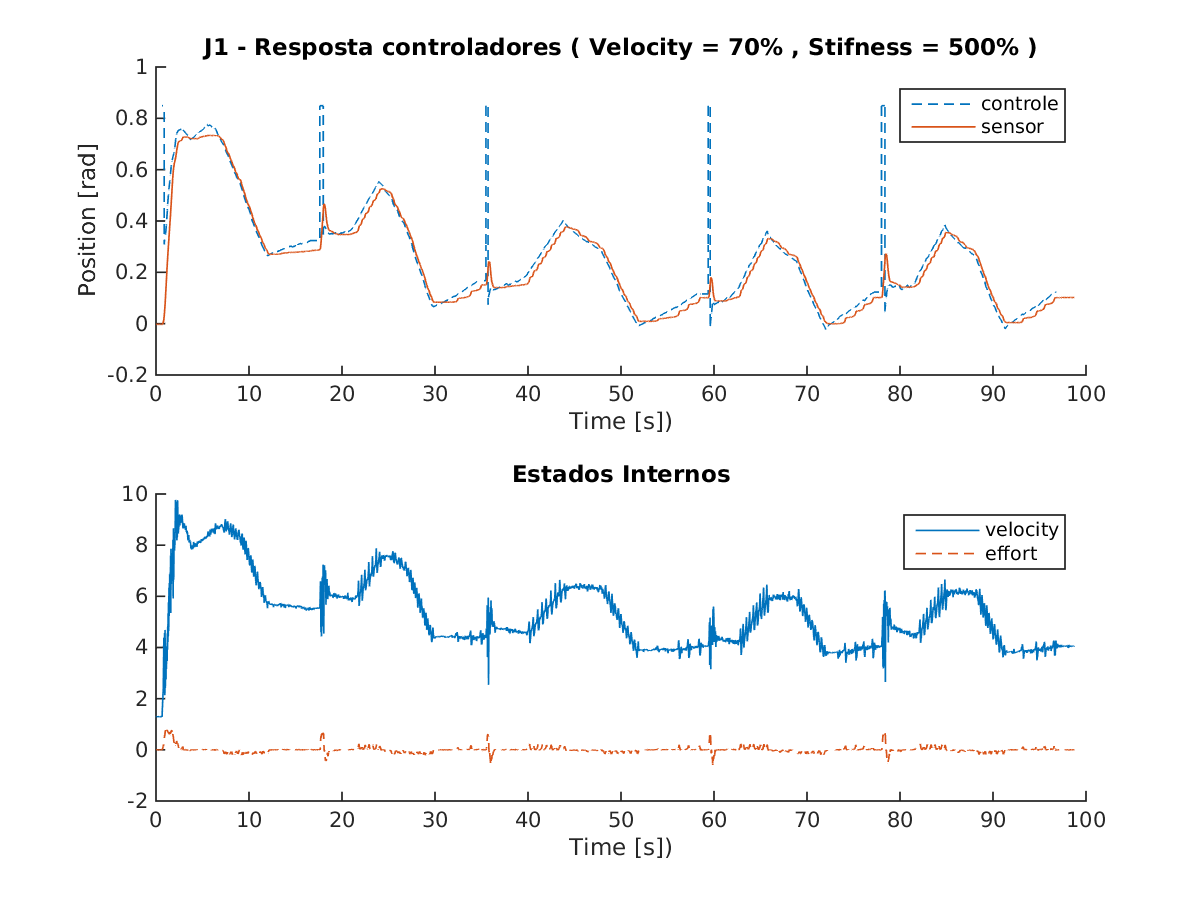
\includegraphics[width = \linewidth]{tex/figs/squareStiffJ3stateEval_J1v70s500.png}
    \label{fig:mekademo}
\end{figure}
\end{column}
\end{columns}
\end{frame}

\begin{frame}{Estudo Trajetória Quadrado}
Resposta Juntas do antebraço e cotovelo
\begin{columns}
\begin{column}{0.5\textwidth}
   \begin{figure}
    \centering
    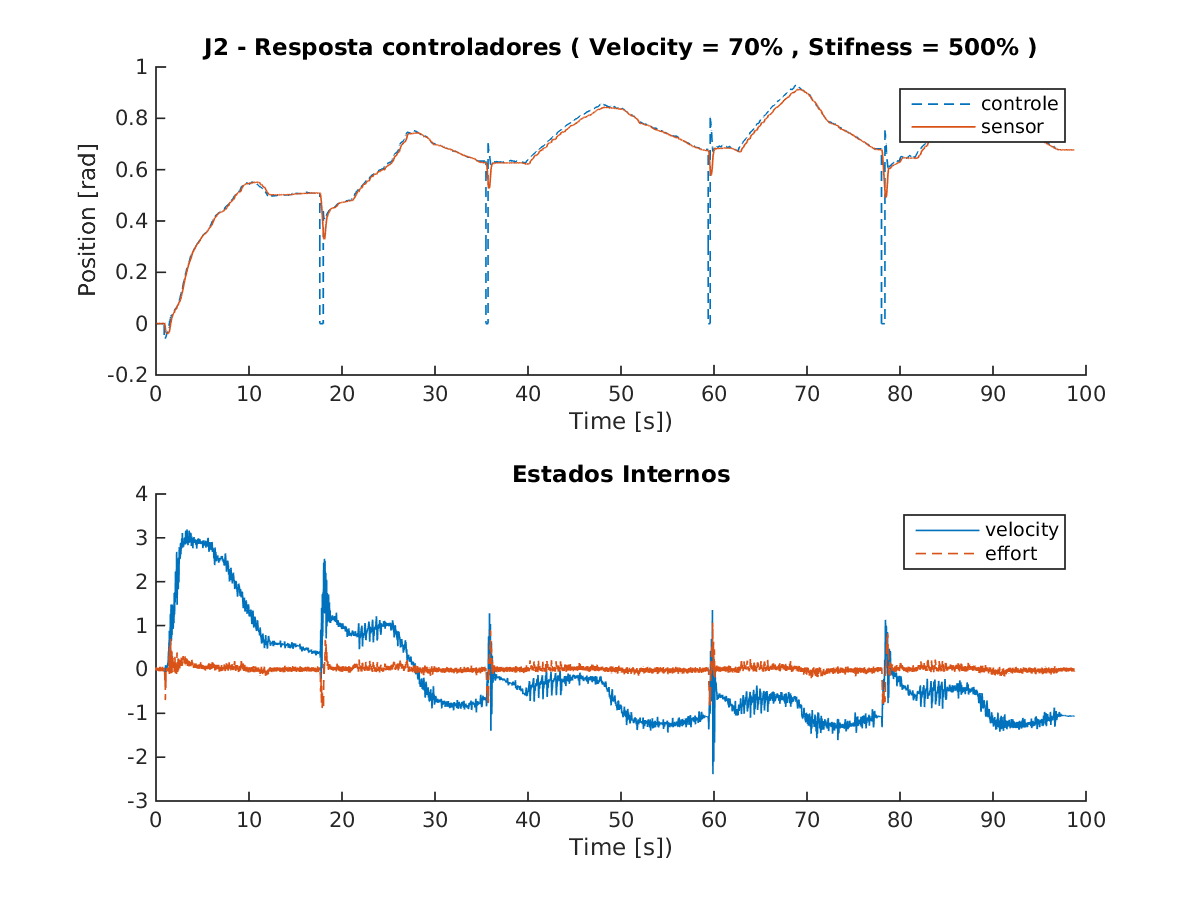
\includegraphics[width = \linewidth]{tex/figs/squareStiffJ3stateEval_J2v70s500.png}
    \label{fig:mekademo}
\end{figure}
\end{column}
\begin{column}{0.5\textwidth}  %%<--- here
    \begin{figure}
    \centering
    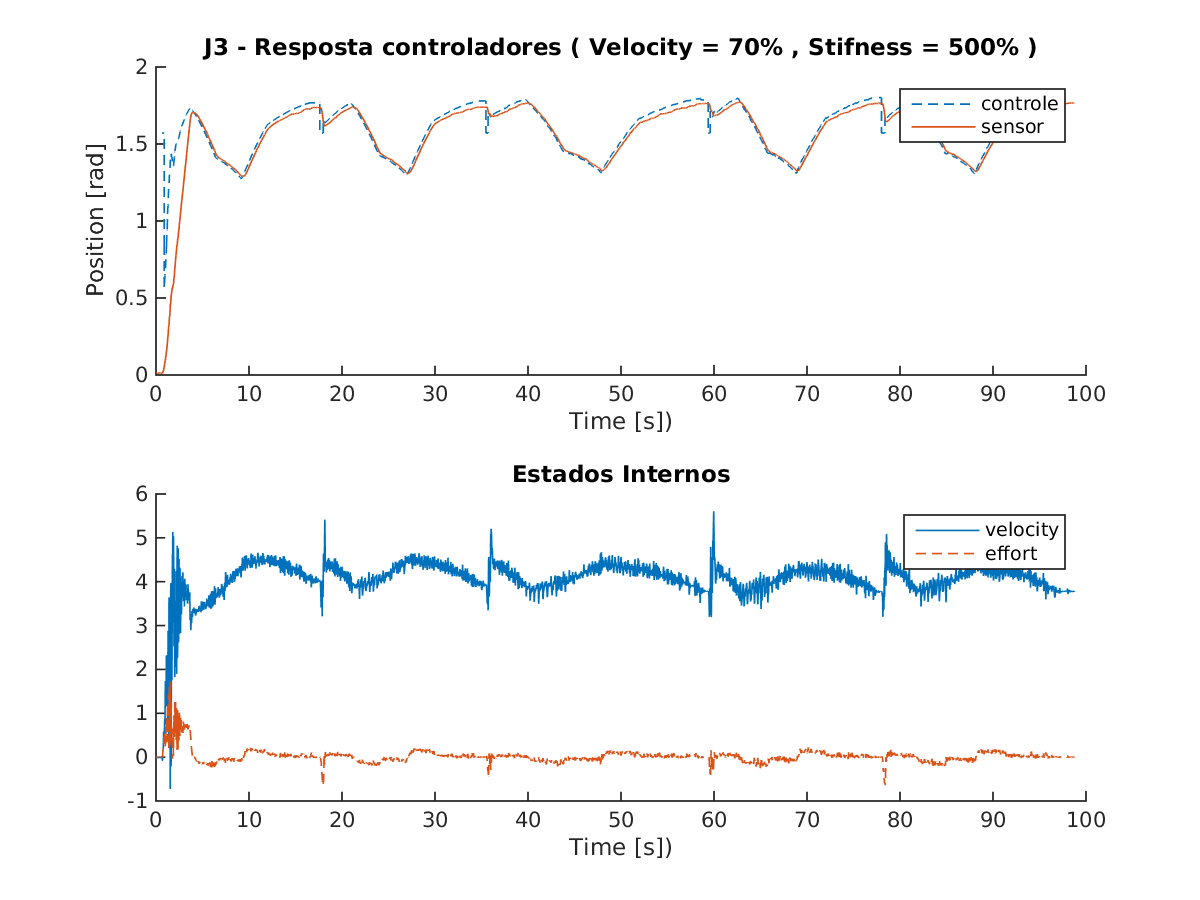
\includegraphics[width = \linewidth]{tex/figs/squareStiffJ3stateEval_J3v70s500.png}
    \label{fig:mekademo}
\end{figure}
\end{column}
\end{columns}
\end{frame}

\begin{frame}{Estudo Trajetória Quadrado}
Resposta Juntas do Pulso
\begin{columns}
\begin{column}{0.5\textwidth}
   \begin{figure}
    \centering
    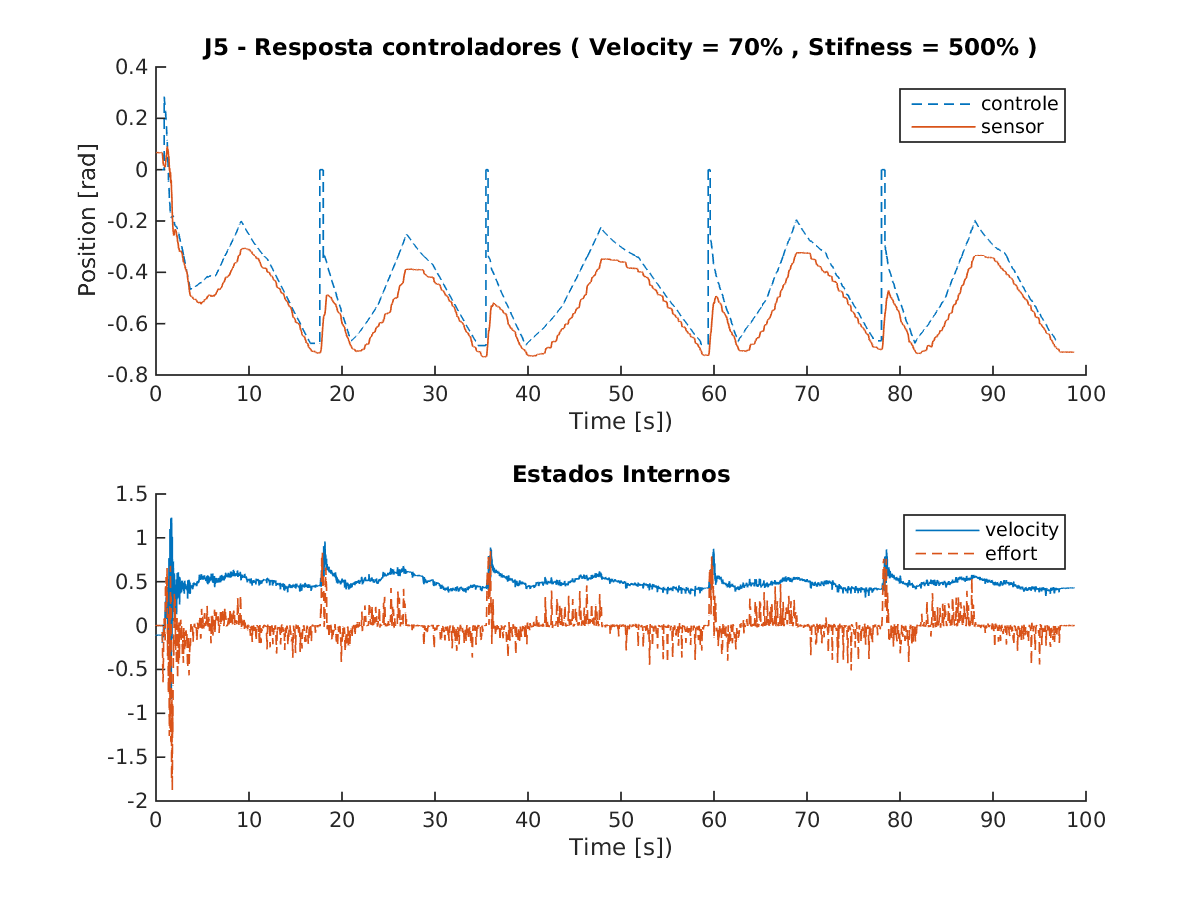
\includegraphics[width = \linewidth]{tex/figs/squareStiffJ3stateEval_J5v70s500.png}
    \label{fig:mekademo}
\end{figure}
\end{column}
\begin{column}{0.5\textwidth}  %%<--- here
    \begin{figure}
    \centering
    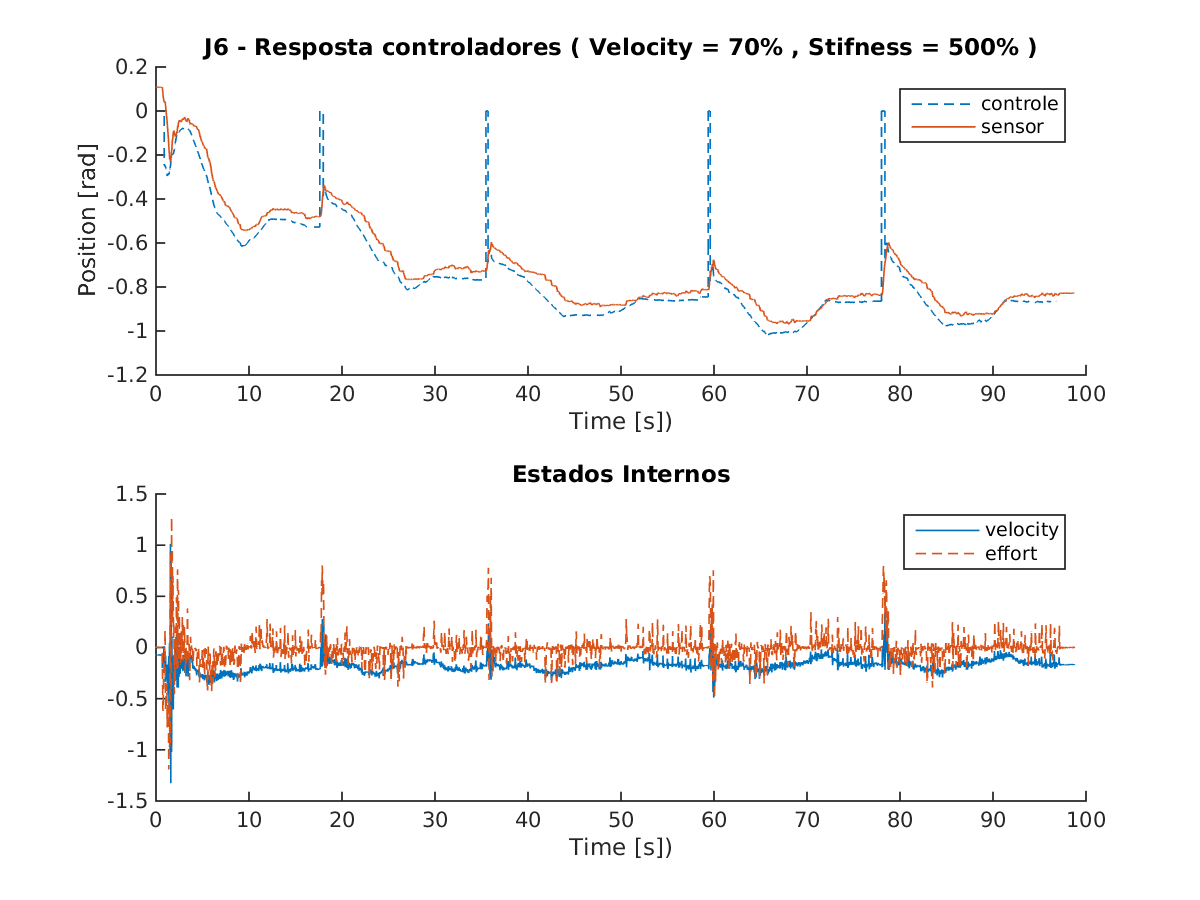
\includegraphics[width = \linewidth]{tex/figs/squareStiffJ3stateEval_J6v70s500.png}
    \label{fig:mekademo}
\end{figure}
\end{column}
\end{columns}
\end{frame}

\begin{frame}{Estudo Trajetória Quadrado}
Resposta Junta do Cotovelo
\begin{figure}
    \centering
    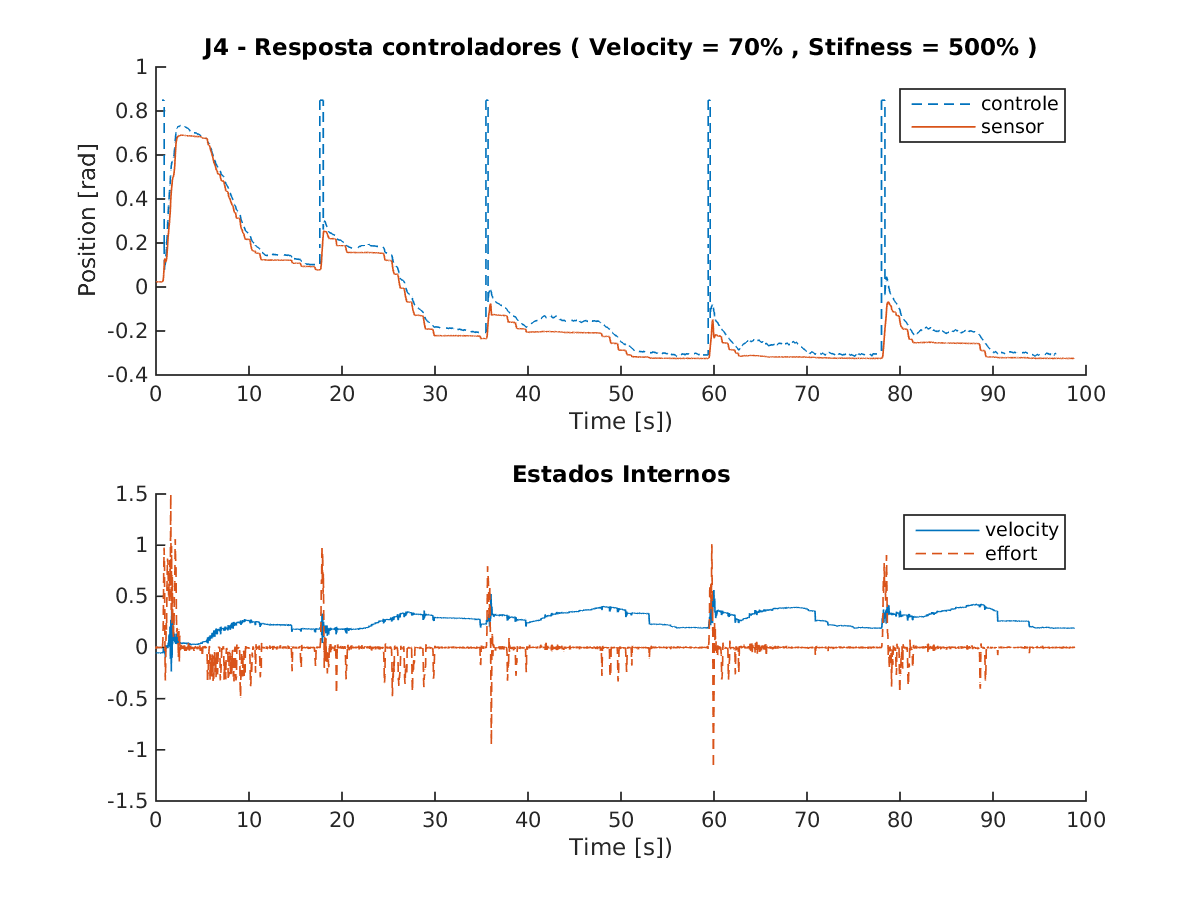
\includegraphics[width = 0.8\linewidth]{tex/figs/squareStiffJ3stateEval_J4v70s500.png}
    \label{fig:mekademo}
\end{figure}
\end{frame}

\begin{frame}{Diagnóstico Meka}
\begin{columns}
\begin{column}{0.5\textwidth}
\begin{itemize}
    \item Orientação distribuída entre o Pulso e o Ombro
    \item Erro maior na orientação
    \item Limitações nos Controladores de Baixo Nível
    \item Limitações nos Atuadores Elásticos
\end{itemize}
\end{column}
\begin{column}{0.5\textwidth}  %%<--- here
\begin{figure}
    \centering
    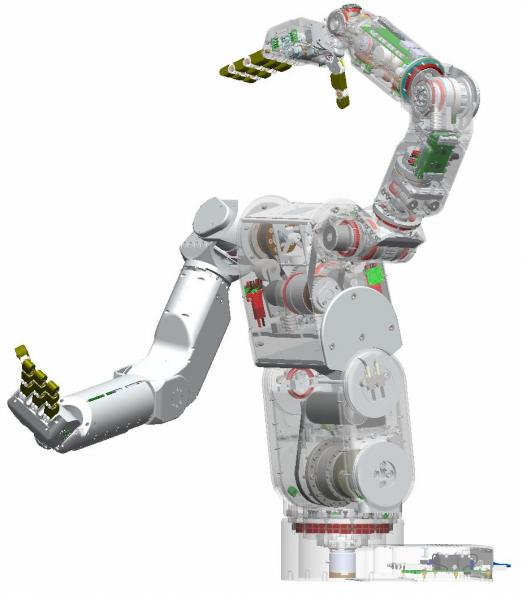
\includegraphics[width = \linewidth]{tex/figs/meka-inside.png}
\end{figure}
\end{column}
\end{columns}
\end{frame}

\section{Conclusão}

\begin{frame}{Conclusão}
\begin{columns}
\begin{column}{0.4\textwidth}
\begin{itemize}
    \item Plataforma de Estudo ( Atuadores Série Elásticos, Filtragem, Sistemas em Tempo Real, ... )
    \item Robótica Colaborativa
\end{itemize}
\end{column}
\begin{column}{0.6\textwidth}  %%<--- here
\begin{figure}
    \centering
    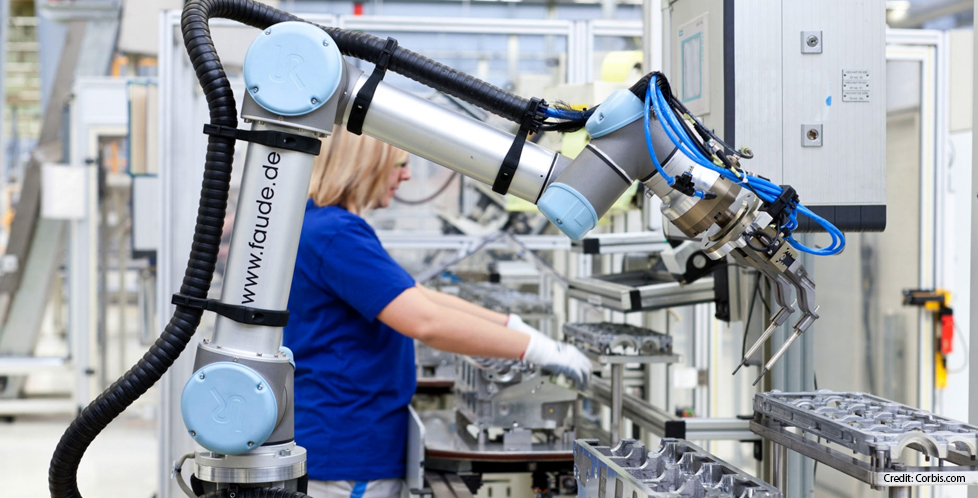
\includegraphics[width = \linewidth]{tex/figs/ur-production.jpg}
\end{figure}
\end{column}
\end{columns}
\end{frame}

\begin{frame}{Trabalhos Futuros}
% Modelagem Matemática
\begin{itemize}
    \item Modelagem do robô e dos fenômenos observados
    \item Controle de Compensação da Gravidade
    \item Filtragem do Sensores
    \item Elasticidade e Amortecimento Virtual
\end{itemize}
\end{frame}

\begin{frame}{}
% Obrigado!
\centering
\Huge{Obrigado!}
\end{frame}

\bibliography{relatorio}

\end{document}